\documentclass[a4paper, fontsize = 8pt, landscape]{scrartcl}
\usepackage{../../../misc_files/LateX/layout_and_colours}
\makeatletter
\def\input@path{{content/lectures/}{content/summary/}{content/examples/}}
\makeatother
\graphicspath{{content/images/}{content/lectures/images/}{content/summary/images/}{content/examples/images/}}

\title{Analysis 1}
\subtitle{Summary}
\author{Jil Zerndt}
\date{HS 2023}

\createtitlepagestyle
\createmainpagestyle
\begin{document}
\begin{multicols}{2}
	\thispagestyle{TitlePageStyle}
	\maketitleinfo
	\sffamily
	


\section{Overview of IT Security}

\mult{2}

\begin{definition}{Key IT Security Goals}
Information security is based on three fundamental principles, commonly known as the CIA triad:
\begin{itemize}
    \item \textbf{Confidentiality} - Ensuring data is only accessible to authorized users
    \item \textbf{Integrity} - Ensuring data is not modified in an unauthorized way
    \item \textbf{Availability} - Ensuring systems and data are accessible when needed
\end{itemize}
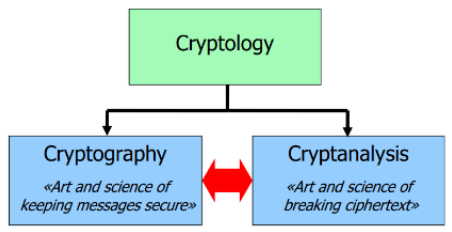
\includegraphics[width=0.6\linewidth]{its_goals.png}
\end{definition}

\begin{concept}{Business IT Risks}
\begin{itemize}
    \item Data loss
    \item System outage
    \item Espionage
    \item Sabotage
    \item Reputation loss
    \item Misuse of computing resources
    \item Violation of regulations
    \item Fraud
    \item Brand misuse
    \item Ransom demands
\end{itemize}
These risks can have significant financial, operational, and reputational impacts.
\end{concept}

\multend

\raggedcolumns

\subsubsection{Security Frameworks and Controls}

\mult{2}

\begin{concept}{Security Control Frameworks}
Security frameworks provide structured approaches to implementing security controls:
\begin{itemize}
    \item \textbf{CIS Controls} - Prioritized set of actions to protect organizations
    \item Controls are typically organized in implementation groups based on difficulty and impact
    \item Focus on preventing the most common attack vectors first
\end{itemize}
\end{concept}

\begin{definition}{Types of Security Measures}
Security measures can be categorized based on their focus:
\begin{itemize}
    \item \textbf{Preventive} - Block threats before they occur (firewalls, access controls)
    \item \textbf{Detective} - Identify when a breach has occurred (IDS, audit logs)
    \item \textbf{Corrective} - Mitigate damage after an incident (backups, incident response)
\end{itemize}
\end{definition}

\multend

\subsubsection{Disaster Recovery}



\begin{concept}{Business Continuity Management}
Disaster recovery and business continuity planning are essential for maintaining availability:
\begin{itemize}
    \item \textbf{Recovery Plan} - Detailed procedures for recovering from incidents
    \item \textbf{Recovery Tests} - Regular testing of recovery procedures
    \item \textbf{Redundancy} - Duplicate systems, power supplies, and network connections
    \item \textbf{Offline backups} - Protection against ransomware and other threats
\end{itemize}
\end{concept}

\begin{KR}{Disaster Recovery Planning}
\paragraph{Initial Assessment}
\begin{itemize}
    \item Identify critical systems and data
    \item Determine acceptable recovery time objectives (RTO)
    \item Determine acceptable recovery point objectives (RPO)
\end{itemize}

\paragraph{Plan Development}
\begin{itemize}
    \item Document recovery procedures
    \item Assign roles and responsibilities
    \item Include contact details for all relevant parties
    \item Develop technical instructions for restoration
\end{itemize}

\paragraph{Testing}
\begin{itemize}
    \item Conduct regular theoretical dry runs
    \item Perform practical tests (e.g., server shutdown, data restoration)
    \item Update procedures based on test results
\end{itemize}

\paragraph{Regular Review}
\begin{itemize}
    \item Review and update plans regularly
    \item Consider changes in infrastructure, personnel, and threats
\end{itemize}
\end{KR}

\begin{example}
A medium-sized company implements a disaster recovery plan for their customer database. They define an RTO of 4 hours and an RPO of 15 minutes, meaning they need to restore service within 4 hours with no more than 15 minutes of data loss. To achieve this, they implement a combination of hourly differential backups with continuous transaction log shipping to a standby site. Regular recovery tests are scheduled quarterly to ensure the plan remains effective.
\end{example}

\mult{2}


\begin{concept}{Problems - Overview}\\ and their impact on data availability
\paragraph{Physisch}
\textbf{unabsichtlich}
\begin{itemize}
    \item Naturkatastrophen
    \item Feuer
    \item Ausfall
    \item Kaffee auf Server
\end{itemize}

\textbf{absichtlich/bösartig}
\begin{itemize}
    \item Feuer
    \item Vandalismus
    \item Garantie läuft aus -> absichtlich langsamer
    \item Social Engineering
\end{itemize}

\paragraph{Virtuell}
\textbf{unabsichtlich}
\begin{itemize}
    \item Bitflip
    \item Config Fehler
    \item Bugs im SW
    \item Phishing klicken
\end{itemize}

\textbf{absichtlich/bösartig}
\begin{itemize}
    \item DDoS
    \item Malware
    \item Ransomware
    \item Phishing senden
    \item Trojaner
\end{itemize}
\end{concept}

\begin{theorem}{Countermeasures - Overview}

\textbf{Disaster Recovery}
    \begin{itemize}
        \item Offline backup solutions
        \item Restoring from images
    \end{itemize}

\textbf{Access Control}
    \begin{itemize}
        \item Restricted Access Rights
        \item Multi-Factor Authentication
        \item Firewalls
        \item Traffic Management Solutions
    \end{itemize}

\textbf{Physical Protection}
    \begin{itemize}
        \item Physical Access Control (locks, fences, etc.)
        \item Fire Protection (extinguishers, alarms, etc.)
        \item Monitoring (CCTV, Guards etc.)
    \end{itemize}

\textbf{Training Processes}
    \begin{itemize}
        \item Employee Training
        \item Four eyes principle
        \item Automation of routine processes
        \item Monitoring
        \item Preventive maintenance
    \end{itemize}

\textbf{Redundancy}
    \begin{itemize}
        \item Uninterruptable Power Supplies
        \item High Availability setups
        \item Load Balancing
        \item Redundant data center
        \item Redundant network connections
    \end{itemize}
\end{theorem}

\multend

\mult{2}

\begin{formula}{Recovery Plan and Test}

    
\includegraphics[width=0.7\linewidth]{recovery_plan_test.png}

    \textbf{Recovery Plan} - description of what to do if something goes wrong
    \begin{itemize}
        \item Roles and responsibilities
        \item Processes
        \item Contact details
        \item Technical instructions
    \end{itemize}

    \textbf{Recovery Test} - testing the recovery plan
    \begin{itemize}
        \item Theoretical dry run
        \item Practical tests
        \begin{itemize}
            \item turn off a server or DC
            \item restore data from backup
        \end{itemize}
    \end{itemize}
\end{formula}

\begin{concept}{Goals of IT Security}

Most measures in Information Security have one of the three following high-level goals:
\begin{itemize}
    \item Ensure data is confidential
    \item Ensure data is not corrupted
    \item Ensure data and systems are available
\end{itemize}

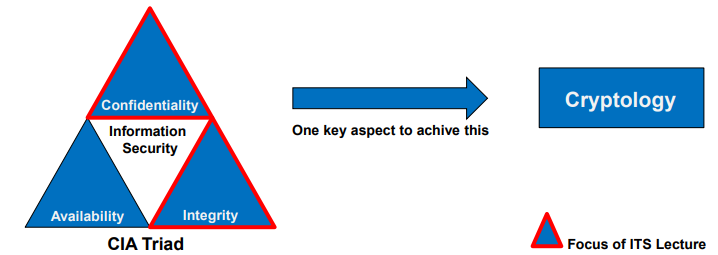
\includegraphics[width=\linewidth]{goals_of_IT_security.png}
\end{concept}

\multend

\raggedcolumns





	\raggedcolumns
	\pagebreak
	\section{Basics}

\subsection{Reelle Zahlen}

\begin{corollary}{Archimedisches Prinzip}
    Sei $x \in \R$ mit $x > 0$ und $y \in \R$. Dann gibt es $n \in \N$ mit $y \leq nx$
\end{corollary}

\begin{theorem}{Ungleichungen}
    $\forall x,y \in \R$
    \begin{equation*}
        \begin{array}{lclc}
            (i) & |x| \geq 0 & (iii) & |x+y| \leq |x| + |y|\\
            (ii) & |xy| = |x||y| & (iv) & |x+y| \geq ||x| - |y||
        \end{array}
    \end{equation*}
\end{theorem}

\begin{theorem}{Young'sche Ungleichung}
       $\forall \varepsilon > 0,~\forall y \in \R$ gilt:
       \hspace{1mm}
       $2 |xy| \leq \varepsilon x^2 + \frac{1}{\varepsilon} y^2$
\end{theorem}

\begin{lemma}{Bernoulli Ungleichung}
    $(1 + x)^n \geq 1 + nx \quad \forall n \in \N, x > -1$
\end{lemma}

\begin{definition}{Kardinalität}
    \begin{itemize}
        \item Mengen $X$, $Y$ heissen \emph{gleichmächtig}, falls es eine \underline{Bijektion} $f: X \to Y$ gibt.
        \item Menge $X$ ist \emph{endlich}, falls entweder $X = \emptyset$ ($\card X = 0$) oder $\exists n \in \N$, sodass $X$ und $\{1,2,\ldots,n\}$ ($\card X = n$) gleichmächtig sind.
        \item Menge $X$ ist \emph{abzählbar}, falls sie endlich oder gleichmächtig wie $\N$ ist.
    \end{itemize}
\end{definition}

\begin{definition}{Beschränktheit}
    $A \subseteq \R$ eine Teilmenge.
    \begin{itemize}
        \item $c \in \R$ ist eine \emph{obere Schranke} von A falls $\forall a \in A: a\leq c$ ($A$ \textit{nach oben beschränkt}).
        \item $c \in \R$ ist eine \emph{untere Schranke} von A falls $\forall a \in A: a \geq c$ ($A$ \textit{nach unten beschränkt}).
        \item $A$ heisst \textit{beschränkt}, wenn nach oben und unten beschränkt.
        \item $m \in \R$ heisst \emph{Maximum} von $A$ falls $m \in A$ und $m$ obere Schranke.
        \item $m \in \R$ heisst \emph{Minimum} von $A$ falls $m \in A$ und $m$ untere Schranke.
    \end{itemize}
\end{definition}

\begin{definition}{Intervalle}
    Ein \emph{abgeschlossenes Intervall} ist eine Teilmenge $I \subseteq \R$ der Form
    \begin{itemize}
        \item Abgeschlossen:
            $[a, b]=\{x \in \mathbb{R} \mid a \leq x \leq b\}$
        \item Offen:
            $(a, b)=\{x \in \mathbb{R} \mid a<x<b\}$
        \item Halboffen:
            $[a, b)=\{x \in \mathbb{R} \mid a \leq x<b\}$
        \item Unendlich:
            $[a, \infty)=\{x \in \mathbb{R} \mid a \leq x\}$
    \end{itemize}
\end{definition}

\subsection{Polynomdivision und Binomialsatz}

\begin{KR}{Polynomdivision}\\
    $\frac{P(x)}{q(x)} = S(x) + \frac{r(x)}{q(x)}$ \qquad $P,q,S,r$ Polynome\\
\emph{!} Vorzeichen von Nullstellen umdrehen.
\tcblower
$$
\begin{array}{cc}
\left(x^3-2 x^2-5 x-6\right):(x-1)=x^2-x-6 & \mid x^3: x=x^2 \\
-\left(x^3-x^2\right) & \mid-x^2: x=-x \\
-x^2-5 x & \\
-\left(x^2-x\right) & \mid-6 x: x=-6 \\
\hline-(-6 x+6) &
\end{array}
$$

Eine Polynomfunktion vom Grad $n$ hat höchstens $n$ reelle Nullstellen.
$$
f(x)=a_n \cdot\left(x-x_1\right) \cdot\left(x-x_2\right) \cdot \ldots \cdot\left(x-x_n\right)
$$
\end{KR}

\begin{theorem}{Binomialsatz}
	$\forall x,y \in \C, n \geq 1$ gilt:
	\\$(x+y)^n = \sum^{n}_{k=0} \begin{pmatrix}n\\k\end{pmatrix} x^k y^{n-k}$\\
\end{theorem}

\subsection{Trigonometrische Funktionen}

\begin{iequation}[align*]
	\tikz[remember picture] \coordinate(sinanchor) at (0,0); \sin x &= \sum_{n=0}^{\infty} \frac{(-1)^n x^{2n + 1}}{(2n+1)!} = x - \frac{x^3}{3!} + \frac{x^5}{5!}\ldots ~ \text{stetig}\\
	\tikz[remember picture] \coordinate(cosanchor) at (0,0); \cos x &= \sum_{n=0}^{\infty} \frac{(-1)^n x^{2n}}{(2n)!} = 1 - \frac{x^2}{2!} + \frac{x^4}{4!}\ldots \hspace{3.8mm} \text{stetig}\\
	\tan x &= \frac{\sin x}{\cos x} \hspace{10mm} \cot x = \frac{\cos x}{\sin x} \tikz[remember picture] \coordinate(trigfunkanchor) at (0,0);
\end{iequation}
\begin{tikzpicture}[remember picture, overlay]
	\node[overlaynote, text width = 28mm, anchor = west] at ($(trigfunkanchor) + (0.5,0.25)$) {$\pi$: kleinste strikt positive Nullstelle von $\sin$.};
	\node[overlaynote, rotate = 90] at ($(trigfunkanchor) + (3,2)$) {$\cos(x) = \sin \left(x + \frac{\pi}{2}\right)$};
	\node[overlaynote, rotate = 20, above left = 3mm and 2mm of sinanchor] (sinnote) {ungerade};
	\draw[overlayarrow] (sinnote) to[bend right] (sinanchor);
	\node[overlaynote, rotate = 20, above left = 3mm and 2mm of cosanchor] (cosnote) {gerade};
	\draw[overlayarrow] (cosnote) to[bend right] (cosanchor);
\end{tikzpicture}

 \begin{center}
    \renewcommand{\arraystretch}{1.3}
    \setlength{\tabcolsep}{4pt}
    \begin{tabular}{|c|c|c|c|c|c|c|c|c|c|}
        \hline
        Grad            & $0^\circ$ & $30^\circ$           & $45^\circ$           & $60^\circ$           & $90^\circ$      & $120^\circ$          & $135^\circ$           & $150^\circ$           & $180^\circ$ \\
        \hline
        $\varphi$       & $0$       & $\frac{\pi}{6}$      & $\frac{\pi}{4}$      & $\frac{\pi}{3}$      & $\frac{\pi}{2}$ & $\frac{2\pi}{3}$     & $\frac{3\pi}{4}$      & $\frac{5\pi}{6}$      & $\pi$       \\
        \hline
        $\sin(\varphi)$ & $0$       & $\frac{1}{2}$        & $\frac{\sqrt{2}}{2}$ & $\frac{\sqrt{3}}{2}$ & $1$             & $\frac{\sqrt{3}}{2}$ & $\frac{\sqrt{2}}{2}$  & $\frac{1}{2}$         & $0$         \\
        \hline
        $\cos(\varphi)$ & $1$       & $\frac{\sqrt{3}}{2}$ & $\frac{\sqrt{2}}{2}$ & $\frac{1}{2}$        & $0$             & $-\frac{1}{2}$       & $-\frac{\sqrt{2}}{2}$ & $-\frac{\sqrt{3}}{2}$ & $-1$        \\
        \hline
        $\tan(\varphi)$ & $0$       & $\frac{\sqrt{3}}{3}$ & $1$                  & $\sqrt{3}$           & $\pm \infty$    & -$\sqrt{3}$          & $-1$                  & $-\frac{\sqrt{3}}{3}$ & $0$         \\
        \hline
    \end{tabular}
\end{center}

\begin{theorem}{Eigenschaften sin/cos}
   \begin{enumerate}
       \item $\exp ix = \cos(x) + i \sin(x) \quad \forall x \in \mathbb{C}$
       \item $\cos x = \cos(-x) ~\text{und}~ \sin(-x) = -\sin x \quad\forall x \in \mathbb{C}$
       \item $\sin(x + y) = \sin(x)\cos(y) + \cos(x)\sin(y)$
       \item $\cos(x + y) = \cos(x)\cos(y) - \sin(x)\sin(y)$
       \item $\cos^2(x) + \sin^2(x) = 1 \quad \forall x \in \mathbb{C}$
       \item $\sin x = \frac{e^{iz} - e^{-iz}}{2i}, \quad \cos x = \frac{e^{iz} + e^{-iz}}{2}$
   \end{enumerate}
\end{theorem}

\begin{corollary}{Winkelverdopplung}\\
        $\sin(2x) = 2 \sin(x)\cos(x)$ \hspace{4mm} $\cos(2x) = \cos^2(x) - \sin^2(x)$
\end{corollary}

\begin{corollary}{Potenz der Winkelfunktion}\\
    %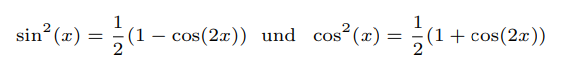
\includegraphics[scale=0.5]{potenz_winkelfunktion.png}
\end{corollary}

\begin{corollary}{Eigenschaften mit $\pi$}
    \begin{enumerate}[itemsep= 2pt]
        \item $e^{i\pi} = -1, \quad e^{2i\pi} = 1$
        \item $\sin\left(x + \frac{\pi}{2}\right) = \cos(x), \quad \cos\left(x + \frac{\pi}{2}\right) = -\sin(x)$
        \item $\sin(x+\pi) = -\sin (x), \quad \sin(x + 2\pi) = \sin(x)$
        \item $\cos(x+\pi) = -\cos (x), \quad \cos(x + 2\pi) = \cos(x)$
    \end{enumerate}
\end{corollary}

\begin{corollary}{Nullstellen}
    \begin{enumerate}
         \item $\text{Nullstellen Sinus} = \{k\cdot \pi : k\in \mathbb{Z}\}$\\
        $\sin(x) > 0 \quad \forall x \in ]2k\pi, ~(2k+1)\pi[, ~ k\in \mathbb{Z}$\\[2pt]
        $\sin(x) < 0 \quad \forall x \in ](2k + 1)\pi, ~(2k+2)\pi[, ~ k\in \mathbb{Z}$
        \item $\text{Nullstellen Cosinus} = \left\{\frac{\pi}{2}+k\cdot \pi : k\in \mathbb{Z}\right\}$\\
        $\cos(x) > 0:\forall x \in \left]-\frac{\pi}{2} +2k\pi, ~-\frac{\pi}{2} +(2k+1)\pi\right[, ~ k\in \mathbb{Z}$\\[2pt]
        $\cos(x) < 0:\forall x \in \left]-\frac{\pi}{2} + (2k + 1)\pi, ~-\frac{\pi}{2} +(2k+2)\pi\right[, ~ k\in \mathbb{Z}$
    \end{enumerate}
\end{corollary}

\noindent Für $\tan(x)$ gilt $x \notin \frac{\pi}{2} + \pi \cdot \Z$ \qquad Für $\cot(x)$ gilt $x \notin \pi \Z$

\begin{theorem}{Bogenlänge}
	Die Bogenlänge einer Kurve, welche im Bereich $[a,b]$ durch eine Funktion $f$ gegeben ist, kann wie folgt berechnet werden.
	\\$L = \int_{a}^{b} \sqrt{1 + ( f'(x) )^2} \dif x$
\end{theorem}

\subsection{Logarithmen und Exponentialfunktionen}

\subsubsection{Logarithmen}
\begin{corollary}{Natürlicher Logarithmus}
   Der nat. Logarithmus $\ln:]0, + \infty[ \to \R$ ist eine streng monoton wachsende, stetige, bijektive Funktion.
\end{corollary}

\begin{corollary}{Rechnen mit Logarithmen}
    \begin{enumerate}
        \item Für $a > 0$ ist $]0, \infty[ \to ]0 + \infty[$ \quad $x \mapsto x^a$ eine stetige, streng monoton wachsende Bijektion.
        \item Für $a < 0$ ist $]0, \infty[ \to ]0 + \infty[$ \quad $x \mapsto x^a$ eine stetige, streng monoton fallende Bijektion.
        \item $\ln (a \cdot b) = \ln a + \ln b \quad \forall a,b \in ]0 +  \infty[$
        \item $\ln (a \div b) = \ln a - \ln b \quad \forall a,b \in ]0 +  \infty[$
        \item ${\ln \left(x^a\right) = a \ln (x) \quad \forall a \in \R, \forall x > 0}$
        \item ${x^a \cdot x^b = x^{a+b} \quad a,b \in \R, \forall x > 0}$
        \item ${\left(x^a\right)^b = x^{a \cdot b} \quad \forall a,b \in \R, \forall x > 0}$
    \end{enumerate}
    Im Allgemeinen gilt: $log_b (a) = \frac{ln(a)}{ln(b)}$
\end{corollary}

%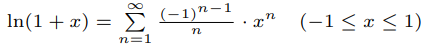
\includegraphics[scale=0.5]{ln.png}

\subsubsection{Werte von log}
\begin{equation*}
	\begin{array}{lccccccc}
		& 0 & 1 & 2 & e & 3 & 5 & 10\\
		\ln & - \infty & 0 & 0.693 & 1 & 1.09 & 1.609 & 2.303\\
		\log_2 & - \infty & 0 & 1 & 1.443 & 1.585 & 2.321 & 3.321\\
		\log_{10} & - \infty & 0 & 0.301 & 0.434 & 0.477 & 0.699 & 1
	\end{array}
\end{equation*}

\subsubsection{Relle Exponentialfunktion}
\begin{center}
    \hfill
    \begin{minipage}{0.3\linewidth}
        \begin{iequation}
            \exp (z) \coloneqq \sum_{n=0}^\infty \frac{z^n}{n!}
        \end{iequation}
    \end{minipage}
    \hfill
    \begin{minipage}{0.6\linewidth}
        \begin{theorem}{Eigenschaften}
            $\exp : \R \to ]0, + \infty[$ ist streng monoton wachsend, stetig und surjektiv.
        \end{theorem}
    \end{minipage}
    \hfill
\end{center}

    \begin{minipage}{0.5\linewidth}
        \begin{iequation}[align*]
            \exp(-x)\exp(x) &= 1\\
	    \text{\textbf{\textsf{}}} \quad\exp(x) &> 0 \qquad\forall x \in \R \tikz[remember picture, overlay]
	    \coordinate(expineq) at (0,0);\\
            \exp(x) &> 1 \qquad\forall x > 0\\
            \exp(a+b) &= \exp(a) \cdot \exp(b)\\
            \exp(a-b) &= \exp(a) \div \exp(b)
        \end{iequation}
\begin{tikzpicture}[overlay, remember picture]
	\node[overlaynote, above right = 8mm and 0mm of expineq] (expineqnote) {Aber nicht: $\exp(z) > 0 \quad \forall z \in \C$};
\end{tikzpicture}
    \end{minipage}
    \hfill
    \begin{minipage}{0.48\linewidth}
        \begin{corollary}
            \\$\exp(z) > \exp(y) \quad \forall z > y$
        \end{corollary}
        \begin{corollary}
            \\${\exp (x) \geq 1 + x \quad \forall x \in \R}$
        \end{corollary}
        \begin{corollary}
            \\$e^{\alpha x} = \sum_{n=0}^\infty \frac{\alpha^n x^n}{n!}$
        \end{corollary}
    \end{minipage}

$\exp(z) = \exp(y + (z-y)) = \exp(y) \exp(z-y)\\
            \exp(x) = \lim_{n\to \infty}(1 + \frac{x}{n})^n$\\
 \begin{minipage}{0.6\linewidth}
        \begin{align*}
            \exp(\ln a + \ln b) &= \exp(\ln a) \cdot \exp (\ln b)\\
            \exp(\ln a)\exp(\ln b) &= ab = \exp(\ln ab)\\
            \exp(\ln a + \ln b) &= \exp(\ln ab)\\
            \ln a + \ln b &= \ln (ab)
        \end{align*}
    \end{minipage}
    \hfill
    \begin{minipage}{0.35\linewidth}
        \begin{iequation}
            x^a \coloneqq \exp(a \ln x)
        \end{iequation}
    \end{minipage}

\subsection{Quadratische Funktionen}

\begin{formula}{Quadratische Funktionen}
$$y=a x^{2}+b x+c$$

    Nullstellen

    \begin{itemize}
      \item $y=a\left(x-x_{1}\right)\left(x-x_{2}\right)$
      \item $x_{0}=\frac{-b \pm \sqrt{b^{2}-4 a c}}{2 a}$
    \end{itemize}

    Scheitelpunkt

    \begin{itemize}
      \item $y=a\left(x-x_{0}\right)^{2}+y_{0}$
      \item $\mathrm{S}=\left(-\frac{b}{2 a}, \frac{4 a c-b^{2}}{4 a}\right)$
    \end{itemize}
\end{formula}

	\raggedcolumns
	\pagebreak
	%\section{Folgen und Reihen}

\subsection{Folgen}

\begin{definition}{Folgen}
    \begin{itemize}
  \item $n \in \mathbb{N}^{*} \rightarrow a_{n} \in \mathbb{R}$
  \item $\left(a_{k}\right)=\left(a_{k}\right)_{k \geq 1}=\left(a_{1}, a_{2}, a_{3}, \ldots, a_{n}, a_{n-1}, \ldots\right)$
\end{itemize}

Die Elemente einer Folge heissen Glieder der Folge $\rightarrow a_{n}$.
\end{definition}

\begin{definition}{Teilfolgen}
    Eine \emph{Teilfolge} einer Folge $\sequence$ ist eine Folge $\sequence[b]$ wobei $b_n = a_{l(n)}$ und $l: \N^* \to \N^*$ eine Abbildung mit der Eigenschaft: $l(n) < l(n+1)~\forall n \geq 1$.
\end{definition}

\begin{definition}{Monotonie}
    \begin{enumerate}
        \item $\sequence$ \emph{monoton wachsend} falls: \null\hfill $a_n \leq a_{n + 1} \quad \forall n \geq 1$.
    	\item $\sequence$ \emph{monoton fallend} falls: \null\hfill $a_n \geq a_{n+1} \quad \forall n \geq 1$.
    \end{enumerate}
\end{definition}

\begin{formula}{Wichtige Folgen}\\
    %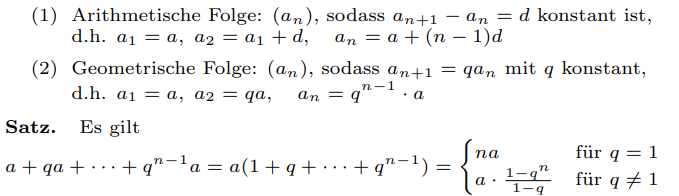
\includegraphics[scale=0.5]{wichtige_folgen.png}
\end{formula}

\begin{remark}
    Folgend sind diese Konzepte beispielhaft vereinfacht.\\
    Abkürzungen
    \begin{itemize}
      \item $A=$ Anfangs-Glied
      \item $d=$ Differenz
      \item $q=$ Quotient
    \end{itemize}
\end{remark}

\begin{definition}{Arithmetische Folge}
$$
a_{k}=(2,3,4,5, \ldots) \rightarrow d=1, A=2
$$

N-tes Glied

$$
a_{n}=A+(n-1) \cdot d
$$

Mittelwert

$$
a_{k}=\frac{a_{k-1}+a_{k+1}}{2}
$$

Partial-Summe

$$
S_{n}=n \cdot \frac{a_{1}+a_{n}}{2}=n \cdot\left(A+\frac{n-1}{2} \cdot d\right)
$$
\end{definition}

\begin{definition}{Geometrische Folge}
$$
a_{k}=\left(\frac{1}{1}, \frac{1}{2}, \frac{1}{4}, \frac{1}{8}, \ldots\right) \rightarrow q=\frac{1}{2}, A=1
$$

N-tes Glied
$$a_{n}=A \cdot q^{n-1}=\frac{A}{q} \cdot q^{n}$$

Mittelwert
$$
\left|a_{k}\right|=\sqrt{a_{k-1} \cdot a_{k+1}}
$$

Partial-Summe

$$
S_{n}=A \cdot \frac{1-q^{n}}{1-q}=A \cdot \frac{q^{n}-1}{q-1}
$$
\end{definition}

\subsection{Grenzwerte und Konvergenz von Folgen}

\begin{definition}{$\varepsilon$-Definition}
    \\Folge $\sequence$ heisst \emph{konvergent}, falls es $l \in \R$ gibt, sodass \vspace{1mm}

    $\forall \varepsilon > 0$ die Menge $\{n \in \N^* : a_n \notin~] l - \varepsilon, l + \varepsilon[\,\}$ endlich ist. ($\N^*$: $\N$/$0$.) \vspace{1mm} \\
    Einfach gesagt: das heisst, dass $|a_n - a| < \epsilon$ ab einem gewissen n für alle $\epsilon$ gilt.

\end{definition}

Bem: $l$ bezeichnet den Grenzwert $\lim_{n \to \infty} a_n$

\begin{definition}{Formelle Grenzwert Definition}
    Folgende Aussagen sind äquivalent:
    \begin{enumerate}
        \item $\sequence$ konvergiert gegen $l = \lim_{n \to \infty} a_n$
        \item $\forall \varepsilon > 0~\exists N \geq 1$, sodass $|a_n -l | < \varepsilon \quad \forall n \geq N$.
    \end{enumerate}
\end{definition}

\begin{lemma}{Einzigartigkeit Grenzwert}
     Es gibt max. ein $l \in \R$ für $a_n$ mit dieser Eigenschaft (max. 1 Grenzwert)
\end{lemma}

\begin{theorem}{Rechenregeln mit Folgen}
    \\Sei $\sequence,\sequence[b]$ konvergente Folgen mit$a = \lim_{n \to \infty} a_n$, $b = \lim_{n \to \infty} b_n$
    \begin{enumerate}
        \item $(a_n \pm b_n)_{n \geq 1}$ konvergent, $\lim_{n \to \infty} (a_n \pm b_n) = a \pm b$.
        \item $(a_n \cdot b_n)_{n \geq 1}$ konvergent, $\lim_{n \to \infty} (a_n \cdot b_n) = a \cdot b$.
        \item $(a_n \div  b_n)_{n \geq 1}$ konvergent, $\lim_{n \to \infty} (a_n \div b_n) = a \div b$.
        \\(solange $b_n \neq 0 ~ \forall n \geq 1$ und $b \neq 0$)
        \item Falls $\exists K \geq 1$ mit $a_n \leq b_n ~ \forall n \geq K$ folgt $a \leq b$.
    \end{enumerate}
\end{theorem}

\begin{highlight}{Spezielle Grenzwerte von Folgen}
    \tcbsubtitle{$n \to \infty$}
    \begin{equation*}
        n^x q^n \to 0 \quad \forall x \in \Z~\text{und}~0 \leq q \leq 1
    \end{equation*}
    \begin{equation*}
         n(\sqrt[n]{x} - 1) \to \ln x \quad \forall x>0
    \end{equation*}
    \begin{equation*}
        \sqrt[n]{a_n} \to 1 ~\text{wenn}~ \lim_{n \to \infty} a_n > 0 ~\text{und}~ \forall a_n > 0
    \end{equation*}
    \begin{center}
        \begin{minipage}{0.3\linewidth}
            \begin{align*}
                \frac{1}{n} &\to 0\\
                1 + \frac{1}{n} &\to 1\\
                \frac{2n}{2^n} &\to 0\\
                \sqrt[n]{n} = n^{\frac{1}{n}} &\to 1\\
                \sqrt[n]{n!} &\to \infty\\
                \frac{1}{n}\sqrt[n]{n!} &\to \frac{1}{e}\\
                \frac{x^n}{n!} &\to 0\\
                \frac{n^n}{n!} &\to \infty
            \end{align*}
        \end{minipage}
        \hfill\vline\hfill
        \begin{minipage}{0.3\linewidth}
            \begin{align*}
                e^n &\to \infty\\
                e^{-n} &\to 0\\
                \frac{e^n}{n^x} &\to \infty\\
                \frac{\sin n}{n} &\to 0\\
                \arctan n &\to \frac{\pi}{2}\\
                ln(n) &\to \infty\\
                \frac{ln(n)}{n} &\to 0\\
                \frac{log(n)}{n - 1} &\to 1
            \end{align*}
        \end{minipage}
        \hfill\vline\hfill
        \begin{minipage}{0.3\linewidth}
            \begin{align*}
                \forall k \in \Q^+ \hspace{2mm}\frac{1}{n^k} &\to 0\\
                \left(1 + n\right)^{\frac{1}{n}} &\to 1\\
                \left(1 + \frac{1}{n}\right)^x &\to 1\\
                \left(1 + \frac{1}{n}\right)^n &\to e\\
                \left(1 + \frac{x}{n}\right)^n &\to e^x\\
                \left(1 - \frac{1}{n}\right)^n &\to \frac{1}{e}\\
                \left(\frac{n}{n + x}\right)^n &\to e^{-x}
            \end{align*}
        \end{minipage}
    \end{center}
    \tcbsubtitle{Divergente Folgen}
    \begin{align*}
        &a_{n}=(-1)^{n}=(-1,1,-1,1,-1 \ldots) \\
        &a_{n}=3+2 n=(5,7,9,11, \ldots)
    \end{align*}
\end{highlight}

\subsection{Tricks und Strategien für Folgen}

\begin{KR}{Konvergenz Folgen}
    \begin{enumerate}
        \item Für Brüche, grösste Potenz von n ausklammern und kürzen. Alle übrigen Brüche der Form $\frac{a}{n^s}$ streichen, da diese zu 0 konvergieren.
        \item Für Wurzeln in einer Summe, multipliziere mit der Differenz der Summe (bei a + b multipliziere mit a - b)
        \item Anwendung Satz von Weierstrass
        \item Anwendung Sandwich-Satz
        \item Vergleich mit Referenz-Folgen (Spezielle Grenzwerte)
        \item Grenzwert durch simple Operationen und Umformen ermitteln
        \item Binom -, Substitutions-, Log-Trick?
        \item Definition der Konvergenz/Limes anwenden
        \item Suchen eines konvergenten Majoranten
    \end{enumerate}
\end{KR}

\begin{KR}{Divergenz Folgen}
    \begin{enumerate}
        \item  Suche einen divergenten Minoranten
        \item Für alternierende Folgen zeige, dass \\$\lim_{n \to \infty} a_p1(n) \neq \lim_{n \to \infty} a_p2(n)$
    \end{enumerate}
\end{KR}

\begin{KR}{Binom Trick}\\
    %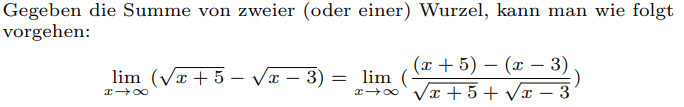
\includegraphics[scale=0.5]{binomtrick.png}
\end{KR}

\begin{KR}{Substitutions Trick}\\
    %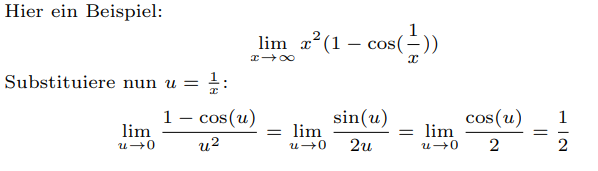
\includegraphics[scale=0.5]{substitutionstrick.png}
\end{KR}

\subsection{Satz von Weierstrass und Sandwich-Satz}

\begin{definition}{Supremum und Infimum}
    $A \subseteq \R, ~A\neq \emptyset$
    \begin{enumerateroman}
        \item $A$ nach oben beschränkt. Dann gibt es eine kleinste obere Schranke von $A$: $c \coloneqq \sup A$. Das \emph{Supremum} von $A$.
        \item $A$ nach unten beschränkt. Dann gibt es eine kleinste untere Schranke von $A$: $c \coloneqq \inf A$. Das \emph{Infimum} von $A$.
    \end{enumerateroman}
    \tcblower
    Vereinfacht formuliert: Für ein abgeschlossenes, halboffenes oder offenes Intervall $[a,b], [a,b), (a,b]$ oder $(a,b)$ gilt $inf = a$, $sup = b$ (solange $a, b \neq \infty$)
\end{definition}

\begin{concept}{Satz von Weierstrass}
    \begin{itemize}
        \item $\sequence$ monoton wachsend und nach oben beschränkt. $\Rightarrow$ $\sequence$ konvergiert mit $\lim_{n \to \infty} a_n = \sup \{a_n : n \geq 1\}$
        \item $\sequence$ monoton fallend und nach unten beschränkt. $\Rightarrow$ $\sequence$ konvergiert mit $\lim_{n \to \infty} a_n = \inf \{a_n : n \geq 1\}$
    \end{itemize}
\end{concept}

\begin{theorem}{Sandwich-Satz}
    Sei $\lim a_n = \alpha$ und $\lim c_n = \alpha$ und $a_n \leq b_n \leq c_n, \forall n \geq k$ dann gilt $\lim b_n = \alpha$\\
    Bmk: k steht hier für eine beliebige natürliche Zahl, ab der die Bedingung immer gilt. Also wie bei der Grenzwert-Definition mit dem <<Gürtel>> um den Grenzwert - das gilt ja auch erst ab einem gewissen Wert n.\\
    Bmk 2: Einfach gesagt heisst das, dass wenn wir den Grenzwert von zwei Folgen bereits kennen und dieser für beide gleich ist, und wir eine dritte Folge haben die <<zwischen>> die zwei bekannten Folgen passt (daher Sandwich-Satz), wissen wir dass auch die dritte Folge den gleichen Grenzwert wie die anderen zwei hat.
\end{theorem}

\subsection{Reihen}

\begin{definition}{Reihen-Konvergenz}
    Die Reihe $\sum_{k = 1}^\infty a_k$ ist \emph{konvergent}, falls die Folge $\sequence[S]$ der Partialsummen konvergiert. In diesem Fall definieren wir: $\sum_{k = 1}^\infty a_k \coloneqq \lim_{n \to \infty} S_n$
\end{definition}

\begin{theorem}{Rechenregeln von Reihen}
    \\Seien $\sum_{k=1}^\infty a_k$ und $\sum_{j=1}^\infty b_j$ konvergent, sowie $\alpha \in \C$.
    \begin{enumerate}
        \item Dann ist $\sum_{k=1}^\infty (a_k + b_k)$ konvergent.\\
            $\sum_{k=1}^\infty (a_k + b_k) = (\sum_{k=1}^\infty a_k) + (\sum_{j=1}^\infty b_j)$.
        \item Dann ist $\sum_{k=1}^\infty \alpha a_k$ konvergent. $\sum_{k=1}^\infty \alpha a_k = \alpha \sum_{k=1}^\infty a_k$
    \end{enumerate}
\end{theorem}

\subsection{Spezielle Reihen}

\begin{highlight}{Spezielle Grenzwerte von Reihen}\\
	\begin{array}{lcl}
		\text{Geom:} & \sum_{k = 0}^\infty a^k & \begin{cases}
		    \frac{1}{1 - a} & |a| < 1\\
		    \text{divergiert} & |a| \geq 1
		\end{cases}\\[10pt]
		& \sum_{k=0}^n ax^k & = a (\frac{1 - x^{n+1}}{1-x})\\[5pt]
		\text{Harm. mit}~b= 1 & \sum_{k = 1}^\infty \frac{1}{k^b} & \begin{cases}
		    \text{konvergiert} & b > 1\\
		    \text{divergiert} & b \leq 1
		\end{cases}\\[10pt]
		\text{Altern. Harm.} & \sum_{k = 1}^\infty \frac{(-1)^{n+1}}{k^b} & \text{konvergiert nach Leibniz}\\[10pt]
		& \sum_{k = 1}^\infty \frac{k^a}{b^k} & \text{abs. konv. falls}~ |b| > 1, k \in \C\\[10pt]
		& \sum_{k = 1}^\infty \frac{k^a}{k!} & \text{abs. konv.}~\forall a \in \C\\[10pt]
	\end{array}
\end{highlight}

\emph{Zeta-Funktion}:
Sei $s > 1$ und $\zeta (s) = \sum_{n=1}^\infty \frac{1}{n^s}$. $\zeta(s)~\text{konvergiert für}~ s> 1$\\
\emph{Teleskopsumme}: Sei $\sum_{k=1}^\infty (a_k - a_{k-1})$. Konvergiert genau dann, wenn $\lim a_n \to g$ konvergiert. Der Grenzwert der Summe ist dann $a_1 -g$.

\subsection{Konvergenzkriterien für Reihen}

\begin{concept} {Nullfolgenkriterium}\\
    $\sum_{k=1}^\infty a_k~\text{konvergiert} \Rightarrow \lim_{k \to \infty} a_k = 0$ aber die Umkehrung stimmt nicht.
\end{concept}

\begin{concept} {Cauchy Kriterium}\\
    Die Reihe $\sum_{k=1}^\infty a_k$ ist genau dann konvergent, falls:\\
    $\forall \varepsilon > 0 ~\exists N \geq 1$ mit $\left|\sum_{k=n}^m a_k \right| < \varepsilon \quad \forall m \geq n \geq N$
\end{concept}

\begin{concept} {Leibniz Kriterium}\\
    Sei $\sequence$ monoton fallend, mit $a_n \geq 0~\forall n \geq 1$ und $\lim_{n \to \infty} a_n = 0$. Dann konvergiert\\
    $S \coloneqq \sum_{k = 1}^{\infty} (-1)^{k+1} a_k$
    und es gilt: $a_1 - a_2 \leq S \leq a_1$.
\end{concept}

\begin{concept} {Majorantenkriterium}\\
    Seien $a_n, b_n \geq 0$ mit $a_n \geq b_n \quad \forall n > n_0$:\\
    $\sum_{n=0}^\infty a_n$ konvergiert $\Rightarrow \sum_{n=0}^\infty b_n$ konvergiert
\end{concept}

\begin{concept} {Minorantenkriterium}\\
    Seien $a_n, b_n \geq 0$ mit $a_n \leq b_n \quad \forall n > n_0$:\\
    $\sum_{n=0}^\infty a_n$ divergiert $\Rightarrow \sum_{n=0}^\infty b_n$ divergiert
\end{concept}

\begin{concept} {Quotientenkriterium}\\
    Sei $\sequence$ mit $a_n \neq 0~\forall n \geq 1$ und: $q = \frac{|a_{n + 1}|}{|a_n|}$\\
    Falls:
    \begin{itemize}
        \item $q < 1$ konvergiert $\sum_{n=1}^\infty a_n$ absolut
        \item $q > 1$ divergiert $\sum_{n=1}^\infty a_n$
    \end{itemize}
    Für $\liminf a_n = 1$ keine Aussage möglich\\
    \emph{!!! für die harmonische Reihe ist dieses Kriterium nicht anwendbar/gültig !!!}
\end{concept}

\begin{concept} {Wurzelkriterium}\\
    Es sei: $q = \sqrt[n]{|a_n|}$\\
    Dann gilt:
    \begin{itemize}
        \item $q < 1 \Rightarrow \sum_{n=1}^\infty a_n$ konvergiert
        \item $q > 1 \Rightarrow \sum_{n=1}^\infty a_n$ und $\sum_{n=1}^\infty |a_n|$ divergieren
        \item $q = 1 \Rightarrow$ keine Aussage möglich
    \end{itemize}
\end{concept}

\begin{KR}{Logarithmus abschätzen}\\
    $\log_b (n)$ kann mit $n^\alpha$ ($\alpha > 0$) abgeschätzt werden.\\
    $\ln(n) \leq \sqrt{n}$
\end{KR}

\begin{KR}{Integral Test}\\
    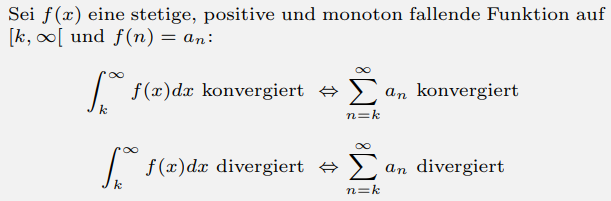
\includegraphics[scale=0.5]{integraltest.png}
\end{KR}

\begin{KR}{Konvergenz Reihen}
    \begin{enumerate}
        \item Handelt es sich um eine spezielle Reihe? (Geometrisch, Teleskopiert, Harmonisch, Zetafunktion)
        \item Ist $\lim a_n$ = 0? (Nullfolgenkriterium)
        \item Ist das Quotientenkriterium oder Wurzelkriterium anwendbar?
        \item Existiert ein konvergierender Majorant / divergirender Minorant?
        \item Kann man das Leibnitzkriterium anwenden?
        \item Integral Test? Partialbruchzerlegung?
    \end{enumerate}
\end{KR}

\begin{center}
    \begin{tikzpicture}[font = \footnotesize]
        \node[draw] (origin) {Gegeben: $\sum_{n=0}^\infty a_n$};
        \matrix (stypes) [
            below = 5mm and 2mm of dstype,
            column sep = 2mm,
            nodes = {
                rectangle,
                draw,
                text width = 18mm,
                minimum height = 12mm
            }
        ] {
            \node[label={[label distance = -4mm]270:geom. Reihe}] (stype1) {$\sum q^n$\\[5pt] $|q| < 1$}; &
            \node[label={[label distance = -4mm]270:altern. Reihe}] (stype2) {$\sum (-1)^n a_n$\\[5pt] $\lim a_n = 0$}; &
            \node[label={[label distance = -4mm]270:Riemann Zeta}] (stype3) {$\zeta (s) = \sum\limits_{n=1}^\infty \frac{1}{n^s}$\\ $s > 1$}; &
            \node[label={[label distance = -4mm]270:Teleskop-Reihe}] (stype4) {$\sum (a_n - a_{n-1})$ \\[5pt] $\exists \lim a_n$}; \\
        };
    \end{tikzpicture}
\end{center}

\subsection{Partialbruchzerlegung bei Reihen}

\noindent Der Grenzwert einer Reihe kann auch mit Partialbruchzerlegung berechnet werden.
\begin{example}
    Was ist der Grenzwert von $\sum_{n=1}^\infty \frac{2}{(n+1)(n+3)}$?
    \tcblower
    \begin{equation*}
        \frac{2}{(n+1)(n+3)} = \frac{a}{n+1} + \frac{b}{n+3} \Rightarrow \begin{cases}
            a + b = 0\\
            3a - b = 2
        \end{cases}
        \quad
        \begin{matrix}
            b = -a = -\frac{1}{2}\\
            a = \frac{1}{2}
        \end{matrix}
    \end{equation*}
    \begin{align*}
        \Rightarrow \sum_{n=1}^\infty \frac{2}{(n+1)(n+3)} &= \frac{1}{2}\sum_{n=1}^\infty\left(\frac{1}{n+1} - \frac{1}{n+3}\right)\\
        & = \frac{1}{2}\left(\frac{1}{2} - \cancel{\frac{1}{4}} + \frac{1}{3} - \cancel{\frac{1}{5}} + \cancel{\frac{1}{4}} - \cancel{\frac{1}{6}} + \ldots\right)\\
        &= \frac{1}{2}\left(\frac{1}{2} + \frac{1}{3}\right) = \frac{5}{2 \cdot 6} = \frac{5}{12}
    \end{align*}
\end{example}

	\raggedcolumns
	\pagebreak
	%\section{Funktionen und Stetigkeit}

\subsection{Eigenschaften von Funktionen}

\begin{definition}{Umkehrfunktion}
    Eine bijektive Funktion $f: D \rightarrow W$ besitzt eine Umkehrfunktion $f^{-1}: W \rightarrow D$.

    \textbf{Vorgehen zum Bestimmen von $f^{-1}$ aus $f(x)=y$:}
    \begin{enumerate}
        \item Nach $x$ auflösen: $x=g(y)$
        \item Variablen vertauschen: $y=g(x)$
    \end{enumerate}
\end{definition}

\begin{theorem}{Operationen von Funktionen}
    Seien $f, g: D \to \R$ zwei Funktionen. Dann sind definiert:
    \begin{itemize}
        \item Addition: $x \rightarrow f(x)+g(x)$
        \item Subtraktion: $x \rightarrow f(x)-g(x)$
        \item Multiplikation: $x \rightarrow f(x) \cdot g(x)$
        \item Division: $x \rightarrow f(x) / g(x)$ (falls $g(x) \neq 0$)
        \item Komposition/Verkettung: $(g \circ f)(x)=g(f(x))$
    \end{itemize}
\end{theorem}

\begin{definition}{Symmetrie}
    Eine Funktion $f: D \to \R$ heisst:
    \begin{itemize}
        \item \textbf{gerade}, falls $f(-x)=f(x)$ für alle $x \in D$
        \item \textbf{ungerade}, falls $f(-x)=-f(x)$ für alle $x \in D$
    \end{itemize}
\end{definition}

\begin{center}
    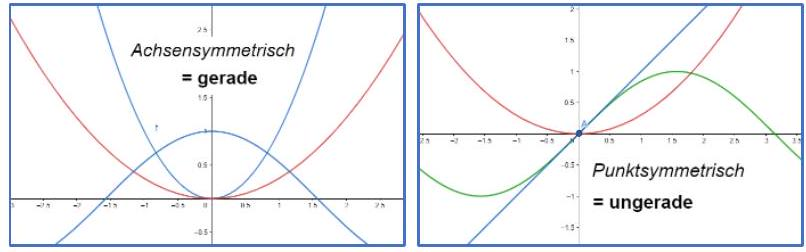
\includegraphics[scale=0.3]{2024_01_20_7bfda6c084929ccc01ffg-01(2).jpg}
\end{center}

\begin{definition}{Beschränktheit}
    Sei $f \in \R^D$.
    \begin{enumerate}
        \item $f$ ist \emph{nach oben beschränkt}, falls $f(D) \subseteq \R$ nach oben beschränkt ist.
        \item $f$ ist \emph{nach unten beschränkt}, falls $f(D) \subseteq \R$ nach unten beschränkt ist.
        \item $f$ ist \emph{beschränkt}, falls $f(D) \subseteq \R$ beschränkt ist.
    \end{enumerate}
\end{definition}

\begin{definition}{Monotonie}
    Eine Funktion $f: D \to \R$ heisst für $x_1, x_2 \in D$ mit $x_1 < x_2$:
    \begin{itemize}
        \item \textbf{monoton wachsend}, falls $f(x_1) \leq f(x_2)$
        \item \textbf{streng monoton wachsend}, falls $f(x_1) < f(x_2)$
        \item \textbf{monoton fallend}, falls $f(x_1) \geq f(x_2)$
        \item \textbf{streng monoton fallend}, falls $f(x_1) > f(x_2)$
    \end{itemize}
\end{definition}

\subsection{Stetigkeit}

\begin{definition}{Stetigkeit}
    Eine Funktion ist stetig, falls:
    \begin{itemize}
        \item die Kurve keine Sprünge macht
        \item man den Graphen der Funktion zeichnen kann, ohne den Stift dabei abzusetzen
    \end{itemize}
\end{definition}

\begin{formula}{Spezielle Stetige Funktionen}
    \begin{enumerate}
        \item $|f|$, $\max(f, g)$ und $\min(f, g)$ sind stetig, falls $f$ und $g$ stetig sind
        \item Polynomielle Funktionen sind auf ganz $\R$ stetig
        \item Die trigonometrischen Funktionen $\sin : \R \to \R$ und $\cos : \R \to \R$ sind stetig
        \item Die Exponentialfunktion $e^x$ ist auf ganz $\R$ stetig
    \end{enumerate}
\end{formula}

\begin{center}
    \begin{tikzpicture}[state/.style={draw, text width = 30mm, align = center, rounded corners = 3pt}]
        \node[state] (ls) {$f$ Lipschitz stetig};
        \node[state, below = 4mm of ls, blue, thick, text = black] (gs) {$f$ gleichmässig stetig};
        \node[state, right = 4mm of gs] (diff) {$f$ differenzierbar};
        \node[state, below = 4mm of gs, blue, thick, text = black] (s) {$f$ stetig};

        \draw[->] (diff) |- (ls) node[midway, above] {Ableitung beschränkt};
        \draw[->] (ls) -- (gs);
        \draw[->, blue, thick] (gs) -- (s);
        \draw[->] (s.west) -- ($(s.west) - (0.25, 0)$) |- (gs) node[pos = 0.25, left] {$\Omega$ kompakt};
    \end{tikzpicture}
\end{center}

\subsection{Grenzwerte von Funktionen}

\begin{highlight}{Wichtige Grenzwerte}
    \begin{center}
        \begin{minipage}{0.4\linewidth}
            \tcbsubtitle{Harmonische Folge:}
            $$\lim_{n \rightarrow \infty} \frac{1}{n}=0$$
            \tcbsubtitle{Geometrische Folge:}
            $$\lim_{n \rightarrow \infty} q^n=0 \quad(|q|<1)$$
        \end{minipage}
        \hfill\vline\hfill
        \begin{minipage}{0.5\linewidth}
            \tcbsubtitle{n-te Wurzel:}
            $$\lim_{n \rightarrow \infty} \sqrt[n]{a}=1$$
            \tcbsubtitle{Eulerzahl:}
            $$\lim_{n \rightarrow \infty}\left(1+\frac{1}{n}\right)^n=e$$
        \end{minipage}
    \end{center}
\end{highlight}

\begin{definition}{Konvergenz einer Funktion}
    Die Funktion $y = f(x)$ hat an der Stelle $x_0$ den Grenzwert $y_0$, falls:

    für jede Folge $(x_n)$ mit $\lim_{n \rightarrow \infty} x_n=x_0$ gilt $\lim_{n \rightarrow \infty} f(x_n)=y_0$.

    \textbf{Bemerkung:} Die Stelle $x_0$ muss nicht im Definitionsbereich $D$ liegen.
\end{definition}

\begin{definition}{Konvergenz und Divergenz}
    \begin{itemize}
        \item \textbf{Konvergenz:} Funktion mit Grenzwert für $x \rightarrow \infty$
        \item \textbf{Divergenz:} Funktion ohne Grenzwert für $x \rightarrow \infty$
        \item \textbf{Bestimmte Divergenz:} Funktion mit $\lim_{x \rightarrow \infty} f(x)= \pm \infty$
    \end{itemize}
\end{definition}

\begin{definition}{Links- und Rechtsseitige Grenzwerte}
    Sei $f : D \to \R$ und $x_0 \in \R$ ein Häufungspunkt. Das bedeutet vereinfacht, dass die Funktion an dieser Stelle evtl. einen Sprung macht, da sich z.B. die Definition ändert.

    \textbf{Beispiel:}
    \begin{equation*}
        f(x) = \begin{cases}
            0 & x < 0\\
            1 & x \geq 0
        \end{cases}
    \end{equation*}

    Setze in diesem Beispiel $x_0 = 0$ und prüfe, ob sich die Funktion von rechts und links dem selben Wert nähert bei $x_0$. (NEIN in diesem Beispiel.)

    \textbf{Formell:} Eine Funktion ist gleichmässig konvergent, wenn für alle Werte gilt:
    $$\lim_{x \to x_0^+} f(x) = \lim_{x \to x_0^-} f(x)$$
    (Linksseitiger Grenzwert = Rechtsseitiger Grenzwert)
\end{definition}

\begin{example2}{Grenzwert einer Funktion}
    Betrachte $f(x)=\frac{x^2-1}{x-1}$ an der Stelle $x_0=1$:

    \begin{center}
        \begin{tabular}{|c|c|c|}
            \hline
            $n$ & $x_n=1-\frac{1}{n}$ & $f(x_n)$ \\
            \hline
            $1$ & 0 & 1 \\
            \hline
            $2$ & 0.5 & 1.5 \\
            \hline
            $3$ & 0.66 & 1.66 \\
            \hline
            $4$ & 0.75 & 1.75 \\
            \hline
            $5$ & 0.8 & 1.8 \\
            \hline
            $10$ & 0.9 & 1.9 \\
            \hline
            $100$ & 0.99 & 1.99 \\
            \hline
            $1000$ & 0.999 & 1.999 \\
            \hline
            $n \rightarrow \infty$ & $x_0=1$ & 2 \\
            \hline
        \end{tabular}
    \end{center}

    Somit gilt: $\lim_{x \rightarrow 1} f(x)=2$
\end{example2}

\subsubsection{Rechnen mit Grenzwerten}

\begin{corollary}{Rechnen mit Grenzwerten von Funktionen}
    Seien $f, g: D \to \R$ Funktionen und existieren die entsprechenden Grenzwerte, dann gilt:
    \begin{itemize}
        \item $\lim_{x \to x_0} (f + g)(x) = \lim_{x \to x_0} f(x) + \lim_{x \to x_0} g(x)$
        \item $\lim_{x \to x_0} (f \cdot g)(x) = \lim_{x \to x_0} f(x) \cdot \lim_{x \to x_0} g(x)$
        \item Sei $f \leq g$, so ist $\lim_{x \to x_0} f(x) \leq \lim_{x \to x_0} g(x)$
        \item Falls $g_1 \leq f \leq g_2$ und $\lim_{x \to x_0} g_1(x) = \lim_{x \to x_0} g_2(x)$, so existiert $\lim_{x \to x_0} f(x) = \lim_{x \to x_0} g_1(x)$
    \end{itemize}
\end{corollary}

\begin{concept}{l'Hospital Regel}
    Seien $f,g : ]a,b[ \to \R$ differenzierbar mit $g'(x) \neq 0$ für alle $x \in ]a,b[$.

    Falls $\lim_{x \to b^-} f(x) = 0$, $\lim_{x \to b^-} g(x) = 0$ und $\lambda \coloneqq \lim_{x \to b^-} \frac{f'(x)}{g'(x)}$ existiert, folgt:
    \begin{iequation}
        \lim_{x \to b^-} \frac{f(x)}{g(x)} = \lim_{x \to b^-}\frac{f'(x)}{g'(x)}
    \end{iequation}
    \tcblower
    \emph{Nur für $\lim_{x \to 0} \frac{f(x)}{g(x)} = \frac{\text{``}0\text{''}}{  \text{``}0\text{''}}$ oder $\frac{\text{``}\infty\text{''}}{\text{``}\infty\text{''}}$ erlaubt.}
\end{concept}

\subsubsection{Strategien und Rechentricks}

\begin{KR}{Erweitern mit $\left(\frac{1}{n^k}\right)$}
    $k=$ höchste Potenz
\end{KR}

\begin{example}
    Beispiel:
    $$
    \begin{aligned}
        \lim_{n \rightarrow \infty} \frac{3 n^2+2 n+1}{5 n^2+4 n+2}
        &\Longrightarrow \textcolor{pink}{\frac{\frac{1}{n^2}}{\frac{1}{n^2}}} \cdot \frac{3 n^2+2 n+1}{5 n^2+4 n+2} \\
        &= \frac{\frac{3 n^2}{n^2}+\frac{2 n}{n^2}+\frac{1}{n^2}}{\frac{5 n^2}{n^2}+\frac{4 n}{n^2}+\frac{2}{n^2}} \\
        &= \frac{3+\frac{2}{n}+\frac{1}{n^2}}{5+\frac{4}{n}+\frac{2}{n^2}}
        = \frac{3+0+0}{5+0+0} = \frac{3}{5}
    \end{aligned}
    $$
\end{example}

\begin{KR}{Erweitern mit $\left(\frac{1}{a^k}\right)$}
    $k=$ höchste Potenz, $a=$ grösste Basis
\end{KR}

\begin{example}
    Beispiel:
    $$
    \begin{aligned}
        \lim_{n \rightarrow \infty} \frac{3^{n+1}+2^n}{3^n+2}
        &\Longrightarrow \textcolor{pink}{\frac{\frac{1}{3^n}}{\frac{1}{3^n}}} \cdot \frac{3 \cdot 3^n+2^n}{3^n+2} \\
        &= \frac{\frac{3 \cdot 3^n}{3^n}+\frac{2^n}{3^n}}{\frac{3^n}{3^n}+\frac{2}{3^n}} \\
        &= \frac{3+\frac{2^n}{3^n}}{1+\frac{2}{3^n}}
        = \frac{3+0}{1+0} = 3
    \end{aligned}
    $$
\end{example}

\begin{KR}{Erweitern mit $\sqrt{a(n)}+\sqrt{b(n)}$}
    Nützlich bei Differenzen von Wurzeln
\end{KR}

\begin{example}
    Beispiel:
    $$
    \begin{aligned}
        &\lim_{n \rightarrow \infty} \sqrt{n^2+n}-\sqrt{n^2-2 n}\\
        &\Longrightarrow \textcolor{pink}{\frac{\sqrt{n^2+n}+\sqrt{n^2-2 n}}{\sqrt{n^2+n}+\sqrt{n^2-2 n}}} \cdot \frac{\sqrt{n^2+n}-\sqrt{n^2-2 n}}{1} \\
        &= \frac{(n^2+n)-(n^2-2 n)}{\sqrt{n^2+n}+\sqrt{n^2-2 n}}
        = \frac{3 n}{\sqrt{n^2+n}+\sqrt{n^2-2 n}}\\
        &= \frac{\frac{1}{n}}{\frac{1}{n}} \cdot \frac{3 n}{\sqrt{n^2+n}+\sqrt{n^2-2 n}} \\
        &= \frac{\frac{3 n}{n}}{\sqrt{\frac{n^2+n}{n^2}}+\sqrt{\frac{n^2-2 n}{n^2}}}
        = \frac{3}{\sqrt{1+\frac{1}{n}}+\sqrt{1-\frac{2}{n}}} \\
        &= \frac{3}{\sqrt{1}+\sqrt{1}} = \frac{3}{2}
    \end{aligned}
    $$
\end{example}

\begin{KR}{Erweitern zur Eulerzahl}
    Forme um zu $\lim_{x \rightarrow \infty}\left(\left(1+\frac{1}{x}\right)^{x}\right)^{a}=e^{a}$
\end{KR}

\begin{example}
    Beispiel:
    $$
    \begin{aligned}
        &\lim_{n \rightarrow \infty}\left(1+\frac{2}{3 n}\right)^{4 n}
        = \left(\left(1+\frac{1}{\frac{3 n}{2}}\right)^{\frac{3 n}{2}}\right)^{a}=e^{a}=e^{\frac{8}{3}}\\
        &\text{Wir rechnen also:}\\
        &4 n=\frac{3 n}{2} \cdot a \text{ und } a=\frac{4 n}{\frac{3 n}{2}}=\frac{8}{3}
    \end{aligned}
    $$
\end{example}

\subsection{Spezielle Sätze}

\begin{definition}{Kompaktes Intervall}
    Ein Intervall $I \subseteq \R$ ist kompakt, falls es von der Form $I=[a,b]$ mit $a \leq b$ ist.
\end{definition}

\textbf{Bemerkung:} Für $x_0$ in einem kompakten Intervall gibt es immer mindestens eine Folge $(a_n)_{n\geq 1}$ mit $a_n \in I$, so dass $\lim_{n \to \infty} a_n = x_0$.

\begin{lemma}{Min-Max Satz}
    Sei $(x_n)$ eine konvergente Folge in $\R$ mit Grenzwert $\lim_{n \to \infty} x_n \in \R$. Sei $a \leq b$. Falls $\{x_n : n \geq 1\} \subseteq [a,b]$, folgt $\lim_{n \to \infty} x_n \in [a,b]$.
\end{lemma}

\begin{theorem}{Minimum-Maximum-Theorem}
    Sei $f:I= [a,b] \to \R$ stetig auf einem kompakten Intervall $I$. Dann gibt es $u \in I$ und $v \in I$ mit:
    \begin{equation*}
        f(u) \leq f(x) \leq f(v) \qquad \forall x \in I
    \end{equation*}
    Insbesondere ist $f$ beschränkt und nimmt ihr Minimum in $u$ und ihr Maximum in $v$ an.
\end{theorem}

\textbf{Zusammen mit dem Zwischenwertsatz folgt:} $f([a,b]) = [f(u), f(v)]$

\begin{lemma}{Zwischenwertsatz}
    Sei $I \subseteq \R$ ein Intervall, $f: I \to \R$ eine stetige Funktion und $a,b \in I$.

    Für jedes $c$ zwischen $f(a)$ und $f(b)$ gibt es ein $z$ zwischen $a$ und $b$ mit $f(z) = c$.
\end{lemma}

\textbf{Bemerkung:} Der Zwischenwertsatz wird oftmals verwendet, um zu zeigen, dass eine Funktion einen gewissen Wert annimmt.

\begin{KR}{Anwendung: Nullstellen}
    \begin{enumerate}
        \item Sei $f:[a,b] \to \R$ stetig. Falls $f(a) \cdot f(b) < 0$, dann $\exists c \in ]a,b[$ mit $f(c) = 0$ (Also eine Nullstelle)
        \item Sei $P(x) = a_n x^n + a_{n-1}x^{n-1} + \ldots + a_0$ ein Polynom mit $a_n \neq 0$ und $n$ ungerade. Dann besitzt $P$ mindestens eine Nullstelle in $\R$
    \end{enumerate}
\end{KR}

\textbf{Gegenbeispiel:} Für $c > 0$ besitzt $Q(x) = x^2 + c$ keine Nullstelle in $\R$.

\begin{center}
    \begin{minipage}{0.44\linewidth}
        Falls eine Funktion wie abgebildet springt, lässt sich der Zwischenwertsatz nicht anwenden.
    \end{minipage}
    \hfill
    \begin{minipage}{0.25\linewidth}
        \begin{equation*}
            f(x) = \begin{cases}
                0 & x < 0\\
                1 & x \geq 0
            \end{cases}
        \end{equation*}
    \end{minipage}
    \hfill
    \begin{minipage}{0.25\linewidth}
        \begin{center}
            \begin{tikzpicture}
                \begin{axis}[
                    axis x line = middle,
                    axis y line = none,
                    ytick style={draw=none},
                    yticklabels={,,},
                    xtick style={draw=none},
                    xticklabels={,,},
                    width = 30mm,
                    ticklabel style = {font=\tiny},
                    ymin = -0.2,
                    ymax = 0.9,
                    xmin = -2,
                    xmax = 2
                ]
                    \filldraw[darkblue] (axis cs: 0,0.75) circle (0.5pt);
                    \addplot[thick, darkblue, ->] coordinates {(-2,0) (0,0)};
                    \addplot[thick, darkblue, ->] coordinates {(0,0.75) (2,0.75)};
                    \begin{pgfonlayer}{bg}
                        \fill[green!30, rounded corners = 1pt] (axis cs: -0.2, 0.85) rectangle (axis cs: 0.2, -0.1);
                    \end{pgfonlayer}
                \end{axis}
            \end{tikzpicture}
        \end{center}
    \end{minipage}
\end{center}

\subsection{Umkehrabbildungen}

\begin{lemma}{Satz über die Umkehrabbildung}
    Sei $I \subseteq \R$ ein Intervall und $f:I \to \R$ stetig und streng monoton.

    Dann ist $J \coloneqq f(I) \subseteq \R$ ein Intervall und $f^{-1}: J \to I$ ist stetig und streng monoton.
\end{lemma}

\begin{center}
    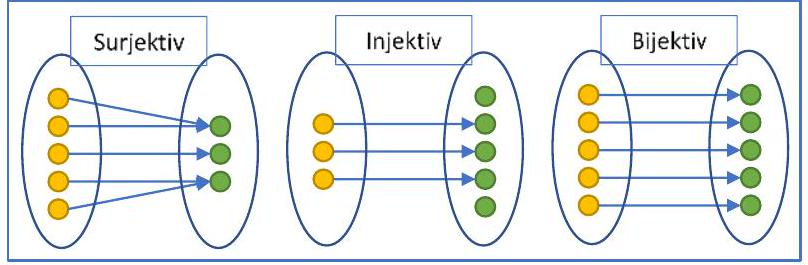
\includegraphics[scale=0.2]{2024_01_20_7bfda6c084929ccc01ffg-01(3).jpg}
\end{center}

\begin{example}
    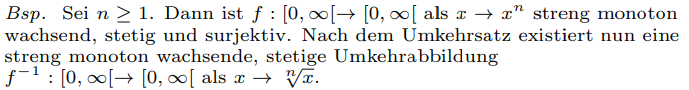
\includegraphics[scale=0.5]{bsp_umkehrabbildung.png}
\end{example}

\subsection{Funktionenfolgen und Funktionenreihen}

Analog zur Folge definieren wir die (reellwertige) \textit{Funktionenfolge} als eine Abbildung $\N \to \R^D$, $n \mapsto f_n$.

Wir bezeichnen $f(n)$ als $f_n$ (n-te Folge) und die Funktionenfolge mit $(f_n)_{n\geq 0}$.

Für jedes $x \in D$ erhält man eine Folge $(f_n(x))_{n \geq 0}$ in $\R$ (wobei $D$ eine Menge ist).

\begin{definition}{Punktweise Konvergenz}
    Die Funktionenfolge $(f_n)_{n\geq 0}$ \emph{konvergiert punktweise} gegen die Funktion $f:D \to \R$, falls für alle $x \in D$ gilt:
    $$f(x) = \lim_{n \to \infty} f_n(x)$$
\end{definition}

\textbf{Warnung:} Nur weil eine Funktionenfolge $(f_n)_{n\geq 0}$ aus stetigen Funktionen besteht, ist die Grenzfunktion $f$ nicht unbedingt stetig.

\begin{definition}{Gleichmässige Konvergenz ($\varepsilon$-Definition)}
    Die Folge $f_n : D \to \R$ \emph{konvergiert gleichmässig} in $D$ gegen $f: D \to \R$, falls gilt:

    $\forall \varepsilon > 0~\exists N \geq 1$, sodass
    \begin{equation*}
        \forall n \geq N, \forall x \in D: |f_n(x) - f(x)| < \varepsilon
    \end{equation*}

    Für Funktionenfolgen: $\forall n,m \geq N$ und $\forall x \in D: |f_n(x) - f_m(x)| < \varepsilon$
\end{definition}

\begin{theorem}{Konvergenz und Stetigkeit}
    Sei $D \subseteq \R$ und $(f_n)_{n\geq 0}$ eine Funktionenfolge aus (in $D$) stetigen Funktionen, die (in $D$) gleichmässig gegen die Funktion $f:D \to \R$ konvergiert.

    Dann ist $f$ (in $D$) stetig.
\end{theorem}

\begin{definition}{Gleichmässige Konvergenz (Limes-Definition)}
    Eine Funktionenfolge $f_n : D \to \R$ ist \emph{gleichmässig konvergent}, falls für alle $x \in D$ der Grenzwert $f(x) \coloneqq \lim_{n \to \infty} f_n(x)$ existiert und die Folge $(f_n)_{n\geq 0}$ gleichmässig gegen $f$ konvergiert.

    Falls $f_n$ eine gleichmässig konvergente Folge stetiger Funktionen ist, dann ist die Funktion $f(x) \coloneqq \lim_{n \to \infty} f_n(x)$ stetig.
\end{definition}

\begin{definition}{Konvergenz von Funktionenreihen}
    Die Reihe $\sum_{k=0}^\infty f_k(x)$ konvergiert gleichmässig (in $D$), falls die durch
    $$S_n(x) \coloneqq \sum_{k=0}^n f_k(x)$$
    definierte Funktionenfolge gleichmässig konvergiert und deren Grenzwert
    $$f(x) \coloneqq \sum_{k=0}^\infty f_k(x)$$
    eine stetige Funktion ist.
\end{definition}

\begin{theorem}{Gleichmässige Konvergenz und Stetigkeit}
    Sei $\sum_{k=0}^\infty c_k x^k$ eine Potenzreihe mit positivem Konvergenzradius $\rho > 0$ und sei:
    \begin{equation*}
        f(x) \coloneqq \sum_{k=0}^\infty c_k x^k \qquad |x| < \rho
    \end{equation*}

    Dann gilt: $\forall 0 \leq r < \rho$ konvergiert $\sum_{k=0}^\infty c_k x^k$ gleichmässig auf $[-r,r]$.

    Insbesondere ist $f:]-\rho, \rho[ \to \R$ stetig. Absolut konvergente Potenzreihen sind stetig.
\end{theorem}

\begin{KR}{Strategie: Konvergenz von Funktionenfolgen}
    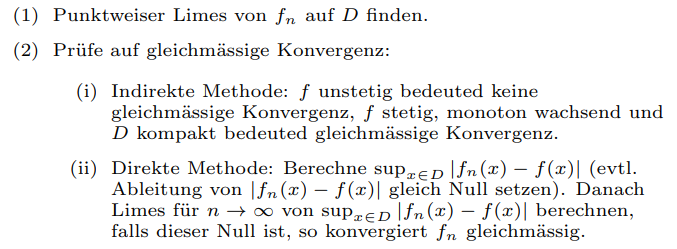
\includegraphics[scale=0.5]{strategie_konvergenz_funktionenfolgen.png}
\end{KR}

\subsection{Konvergenzradius}

\subsubsection{Potenzreihe und Konvergenzradius}

\begin{definition}{Potenzreihe}
    Eine Potenzreihe ist eine Reihe von der Form $\sum_{k=0}^\infty c_k z^k$, wobei $(c_k)_{k\geq 0}$ eine Folge ist.
\end{definition}

\begin{corollary}{Konvergenz und Divergenz}
    Die Potenzreihe $\sum_{k=0}^\infty c_k z^k$ konvergiert absolut für alle $|z| < \rho$ und divergiert für alle $|z| > \rho$.
\end{corollary}

Der Konvergenzradius ($\rho$) gibt an, in welchem Bereich von $\R$ bzw. $\C$ die Konvergenz garantiert ist. Die Potenzreihe hat \emph{positiven Konvergenzradius}, falls $\limsup_{k \to \infty} \sqrt[k]{|c_k|}$ existiert.

Der Konvergenzradius ist dann definiert als:
\begin{equation*}
    \rho = \begin{cases}
        + \infty & \text{falls}~\limsup_{k \to \infty} \sqrt[k]{|c_k|} = 0\\
        \frac{1}{\limsup_{k \to \infty} \sqrt[k]{|c_k|}} & \text{falls}~\limsup_{k \to \infty} \sqrt[k]{|c_k|} > 0
    \end{cases}
\end{equation*}

Alternativ lässt sich der Konvergenzradius auch mit $\rho = \lim_{n \to \infty} \left| \frac{a_n}{a_{n+1}} \right|$ berechnen.

	\raggedcolumns
	\pagebreak
	%\section{Differentialrechnung}

\subsection{Differenzierbarkeit}

\begin{definition}{Sekanten-Steigung und Differentialquotient}
    Sei $f$ eine Funktion und $\left[x_{0}, x_{0}+h\right]$ ein Intervall im Definitionsbereich von $f$. Der Quotient

    $$\frac{\Delta f}{\Delta x}=\frac{f\left(x_{0}+h\right)-f\left(x_{0}\right)}{h}$$

    heisst Differentialquotient von $f$.
\end{definition}

\begin{center}
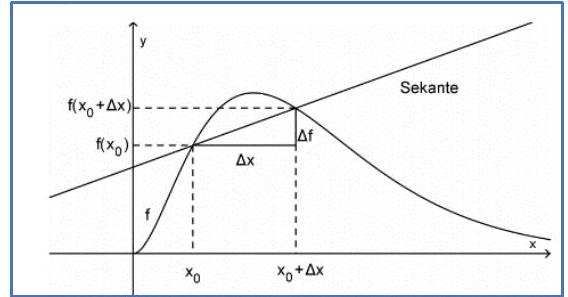
\includegraphics[scale=0.3]{2024_01_20_7bfda6c084929ccc01ffg-03.jpg}
\end{center}

\begin{definition}{Differenzierbarkeit}
    $f$ ist in $x_0$ \emph{differenzierbar}, falls der Grenzwert $\lim_{x \to x_0} \frac{f(x) -f(x_0)}{x -x_0}$
    existiert.

    Ist dies der Fall, wird der Grenzwert mit $f'(x)$ bezeichnet:
    $$
    f'(x_0) = \lim_{h \to 0}\frac{\Delta f}{\Delta x} = \lim_{h \to 0}\frac{f(x_0 + h) -f (x_0)}{h}
    $$
    Den Grenzwert selbst bezeichnet man als Ableitung.
    \tcblower
    Vereinfacht: Eine Funktion ist differenzierbar, falls die Kurve keine Knicke macht.
\end{definition}

\begin{formula}{Tangentengleichung}
    $$
    y=f^{\prime}\left(x_{0}\right) \cdot\left(x-x_{0}\right)+f\left(x_{0}\right)
    $$
\end{formula}

\begin{definition}{Stetige Differenzierbarkeit}
	Eine Funktion ist stetig differenzierbar, wenn sie differenzierbar ist und ihre Ableitungsfunktion stetig ist.
\end{definition}

\begin{definition}{n-fache Differenzierbarkeit}
	\begin{enumerate}
		\item Für $n \geq 2$ ist $f$ \emph{$n$-mal differenzierbar} in $D$ falls $f^{n-1}$ in $D$ differenzierbar ist. Dann ist $f^{(n)} \coloneqq \left(f^{(n-1)}\right)'$ und nennnt sich die $n$-te Ableitung von $f$.
		\item Die Funktion $f$ ist \emph{$n$-mal stetig differenzierbar} in $D$, falls sie $n$-mal differenzierbar ist und falls $f^{(n)}$ in $D$ stetig ist.
		\item Die Funktion $f$ ist in $D$ \emph{glatt}, falls sie $\forall n \geq 1$, $n$-mal differenzierbar ist.
	\end{enumerate}
\end{definition}

\begin{remark}
    Beispiele glatter Funktionen:
    \begin{itemize}
	    \item $\exp$, $\sin$, $\cos$, $\sinh$, $\cosh$, $\tanh$ sind glatt auf $\R$
	    \item Alle Polynome sind auf ganz $\R$ glatt
	    \item $\ln : ]0, + \infty[ \to \R$ ist glatt
    \end{itemize}
\end{remark}

\subsection{Ableitungen}

\subsubsection{Ableitungsregeln}

\begin{concept}{Ableitungsregeln}
    Seien $f,g: D \to \R$  differenzierbar. Dann gelten:
    \begin{itemize}
        \item Summe/Differenz: $$(f + g)'(x) = f'(x) + g'(x)$$
        \item Produkt: $$(f \cdot g)'(x) = f'(x)g(x) + f(x)g'(x)$$
        \item Quotient: $$\left(\frac{f}{g}\right)'(x) = \frac{f'(x) g(x) - f(x) g'(x)}{g(x)^2}$$
        \item Kettenregel: $$(g \circ f)' (x) = g'(f(x)) f'(x)$$
        \item Umkehrfunktion: $$\left(f^{-1}\right)'(y_0) = \frac{1}{f'(x)}$$
        \item Potenz/Logarithmus:
        $$(a^{f(x)})' = \ln(a) \cdot a^{f(x)} \cdot f'(x)$$
        $$(f(x)^{g(x)})' = f(x)^{g(x)} \cdot (\ln(f(x)) \cdot g(x))' =  f(x)^{g(x)} \cdot \left(\ln(f(x)) \cdot g'(x) + g(x) \cdot \frac{f'(x)}{f(x)}\right)$$
    \end{itemize}
\end{concept}

\subsubsection{Grundlegende Ableitungen}

\begin{formula}{Potenzfunktionen}
    $$f(x)=x^{n} \quad \Rightarrow \quad f^{\prime}(x)=n \cdot x^{n-1}$$
\end{formula}

\begin{formula}{Exponentialfunktionen}
    $$
    \begin{array}{ll}
    f(x)=a^{x} & f^{\prime}(x)=a^{x} \cdot \ln (a) \\
    f(x)=e^{x} & f^{\prime}(x)=e^{x}
    \end{array}
    $$
\end{formula}

\begin{formula}{Logarithmusfunktionen}
    $$
    \begin{array}{ll}
    f(x)=\ln (x) & f^{\prime}(x)=\frac{1}{x} \\
    f(x)=\log _{a}(x) & f^{\prime}(x)=\frac{1}{\ln (a) \cdot x}
    \end{array}
    $$
\end{formula}

\begin{formula}{Trigonometrische Funktionen}
    $$
    \begin{array}{ll}
    \sin'(x) = \cos(x) & \cos'(x) = -\sin(x) \\
    \tan'(x) = \frac{1}{\cos^{2}(x)} = 1+\tan^{2}(x) & \cot'(x) = -\frac{1}{\sin^{2}(x)} = -1-\cot^{2}(x)
    \end{array}
    $$
\end{formula}

\begin{formula}{Arkusfunktionen}
    $$
    \begin{aligned}
    \arcsin^{\prime}(x) & =\frac{1}{\sqrt{1-x^{2}}} \\
    \arccos^{\prime}(x) & =\frac{-1}{\sqrt{1-x^{2}}} \\
    \arctan^{\prime}(x) & =\frac{1}{1+x^{2}}
    \end{aligned}
    $$
\end{formula}

\begin{formula}{Hyperbolische Funktionen}
    $$
    \begin{array}{ll}
    \sinh'(x) = \cosh(x) & \cosh'(x) = \sinh(x)
    \end{array}
    $$
\end{formula}

\begin{remark}
    Für gerade $k$ gilt $\cosh (x)^{(k)}=\cosh (x)$ und für ungerade $k$ gilt $\cosh (x)^{(k)}=\sinh (x)$, analoges gilt für $\sinh$.
\end{remark}

\subsubsection{Weitere nützliche Ableitungen}

\begin{formula}{Weitere Ableitungen}
    $$
    \begin{array}{ll}
    \left(\frac{1}{x^n}\right)' = \frac{-n}{x^{n+1}} & \left(\sqrt[n]{x}\right)' = \frac{1}{n\sqrt[n]{x^{n-1}}} \\
    (x^x)' = x^x(1+\ln x) & (|x|)' = \sgn(x) \quad (x \neq 0)
    \end{array}
    $$
\end{formula}

\begin{center}
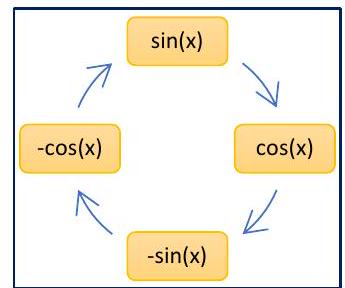
\includegraphics[scale=0.25]{2024_01_20_7bfda6c084929ccc01ffg-05.jpg}
\end{center}

\subsection{Höhere Ableitungen}

\begin{theorem}{Rechnen mit höheren Ableitungen}
	Sei $D \subseteq \R$, $n \geq 1$ und $f,g: D \to \R$ $n$-mal differenzierbar in $D$.
	\begin{enumerate}
		\item $f+g$ ist $n$-mal differenzierbar und $(f + g)^{(n)} = f^{(n)} + g^{(n)}$
		\item $f \cdot g$ ist $n$-mal differenzierbar und $(f \cdot g)^{(n)} = \sum_{k=0}^n \binom{n}{k} f^{(k)} g^{(n-k)}$ (Leibniz-Regel)
        \item $\frac{f}{g}$ ist $n$-mal differenzierbar falls $g(x) \neq 0, \forall x \in D$
        \item $(g \circ f)$ ist $n$-mal differenzierbar
	\end{enumerate}
\end{theorem}

\subsubsection{Zentrale Sätze der Ableitungsrechnung}

\begin{theorem}{Satz von Rolle}
    Sei $f:[a,b] \to \R$ stetig in $]a,b[$ differenzierbar. Erfüllt sie $f(a) = f(b)$ so gibt es $\xi \in ]a,b[$ mit $f'(\xi) = 0$.

    \tcblower
    $\xi$ bezeichnet eine Extremalstelle im Intervall $]a,b[$.
\end{theorem}

\begin{theorem}{Lagrange (Mittelwertsatz)}
    Sei $f:[a,b] \to \R$ stetig mit $f$ in $]a,b[$ differenzierbar. Dann gibt es $\xi \in ]a,b[$ mit
    $$f(b) - f(a) = f'(\xi) (b-a)$$

    \tcblower
    $f'(\xi)$ ist die Steigung der Sekante zwischen $(a, f(a))$ und $(b, f(b))$:
    $$f'(\xi) = \frac{f(b) - f(a)}{b - a}$$
\end{theorem}

\begin{theorem}{l'Hospital}
    Seien $f,g : [a,b] \to \R$ stetig und in $]a,b[$ differenzierbar. Dann gibt es $\xi \in ]a,b[$ mit
    $$g'(\xi)\left(f(b) - f(a)\right) = f'(\xi) \left(g(b) - g(a)\right)$$

    Falls $g'(x) \neq 0 \quad \forall x \in ]a,b[$ folgt $g(a) \neq g(b)$ und
    $$\frac{f(b) - f(a)}{g(b) - g(a)} = \frac{f'(\xi)}{g'(\xi)}$$
\end{theorem}

\subsection{Kurvendiskussion}

\subsubsection{Monotonie und Krümmung}

\begin{definition}{Monotonie}
    Sei $y=f(x)$ eine differenzierbare Funktion in $D$ mit $x_{0} \in D$.
    \begin{itemize}
        \item $f'(x_{0}) = 0$ $\Rightarrow$ $f$ konstant, bzw. horizontale Tangente
        \item $f'(x_{0}) > 0$ $\Rightarrow$ $f$ streng monoton wachsend
        \item $f'(x_{0}) < 0$ $\Rightarrow$ $f$ streng monoton fallend
    \end{itemize}
\end{definition}

\begin{theorem}{Krümmung}
    Zusammenhang zwischen 2. Ableitung und Krümmung:
    \begin{itemize}
      \item $f^{\prime \prime}\left(x_{0}\right)>0$ $\Rightarrow$ Konvex (linksgekrümmt, nach oben geöffnet)
      \item $f^{\prime \prime}\left(x_{0}\right)<0$ $\Rightarrow$ Konkav (rechtsgekrümmt, nach unten geöffnet)
      \item $f^{\prime \prime}\left(x_{0}\right)=0$ $\Rightarrow$ Keine eindeutige Krümmung
    \end{itemize}
\end{theorem}

\begin{remark}
    Die Summe zweier konvexer Funktionen ist konvex. (Für konkave Funktionen gilt dies analog.)
\end{remark}

\begin{center}
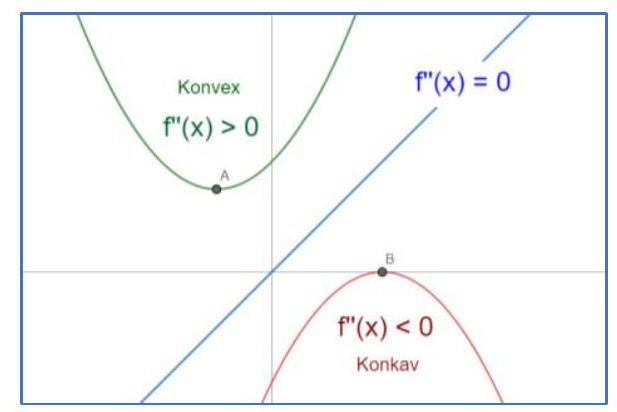
\includegraphics[scale=0.2]{2024_01_20_7bfda6c084929ccc01ffg-07.jpg}
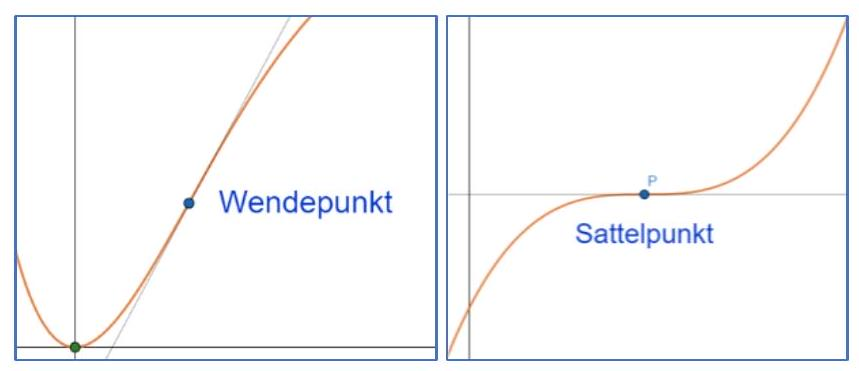
\includegraphics[scale=0.15]{2024_01_20_7bfda6c084929ccc01ffg-08.jpg}
\end{center}

\subsubsection{Relative Extrema}

\begin{definition}{Relative Extrema}
    \begin{itemize}
      \item Relative Extremal-Stelle $x_0$ $\Longrightarrow$ Minimal-/Maximalstelle
      \item Relatives Extremum $y_0$ $\Longrightarrow$ Maximum/Minimum
      \item Relativer Extremal-Punkt $P_0 = (x_0, y_0)$ $\Longrightarrow$ Hoch-/Tiefpunkt
    \end{itemize}
\end{definition}

\begin{center}
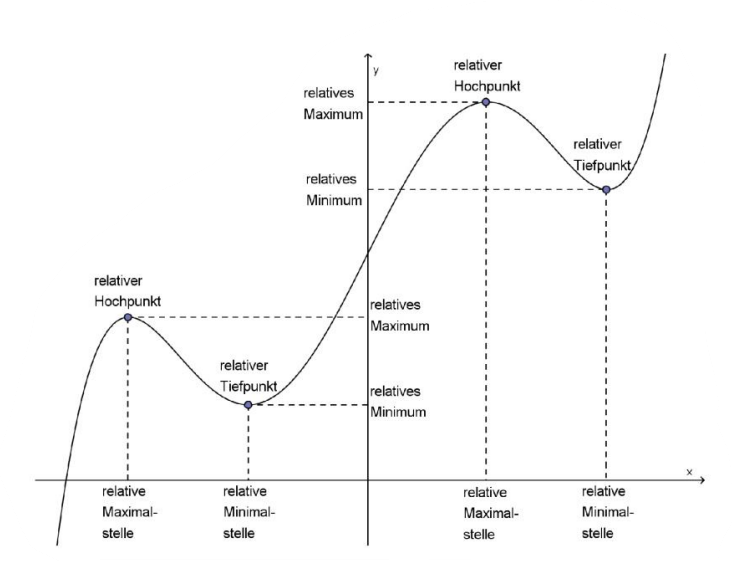
\includegraphics[scale=0.45]{relative maxima.png}
\end{center}

\begin{KR}{Vorgehen relative Extrema}
    Bestimmung relativer Extrema von $f(x) = y$:
    \begin{enumerate}
	    \item Bestimme $f'(x)$ (Erste Ableitung)
	    \item Bestimme Nullstellen von $f'(x)$: $f'(x) = 0 \Rightarrow x$ lokales Extremum
	    \item Bestimme $f''(x)$ (Zweite Ableitung)
		    \begin{itemize}
			    \item $f''(x) = 0$ $\Rightarrow$ siehe Allgemeines Kriterium
			    \item $f''(x) < 0$ $\Rightarrow$ relatives Maximum (Hochpunkt)
			    \item $f''(x) > 0$ $\Rightarrow$ relatives Minimum (Tiefpunkt)
		    \end{itemize}
        \item In Gleichung $f(x) = y$ einsetzen für Punkt $P(x, y)$
    \end{enumerate}
\end{KR}

\begin{example}
    $$f(x)=x^{5}-\frac{65}{3} x^{3}+180 x$$

    \begin{enumerate}
        \item $f'(x)=5 x^{4}-65 x^{2}+180$
        \item $f'(x)=0 \Rightarrow x_{0}=2 \pm \sqrt{3}$
        \item $f''(x)=20 x^{3}-130 x$
        \item Einsetzen:
            \begin{itemize}
              \item $f^{\prime \prime}(2-\sqrt{3})=-34 < 0 \Rightarrow$ Maximum
              \item $f^{\prime \prime}(2+\sqrt{3})=554 > 0 \Rightarrow$ Minimum
            \end{itemize}
        \item Hochpunkt/Tiefpunkt: $P\left(x_{0}, f(x_0)\right)$
    \end{enumerate}
\end{example}

\subsubsection{Wende- und Sattelpunkte}

\begin{definition}{Wende- und Sattelpunkte}
    Als Wendepunkte werden Punkte bezeichnet bei denen sich der Drehsinn (die Krümmung) ändert.

    Wendepunkte mit horizontaler Tangente werden als Sattelpunkte oder Terrassenpunkte bezeichnet.

    Die Tangente an einem Wendepunkt heisst Wendetangente.
\end{definition}

\begin{KR}{Berechnung Wendepunkte}
    Ermittlung durch Lösen der Gleichung $f^{\prime \prime}(x)=0 \rightarrow x_{0}$.

    Bedingungen (sei $y=f(x)$ dreimal differenzierbar):
    \begin{itemize}
      \item $f^{\prime \prime}\left(x_{0}\right)=0$
      \item $f^{(3)}\left(x_{0}\right) \neq 0$ $\Rightarrow$ Wendepunkt
      \item Falls zusätzlich $f^{\prime}\left(x_{0}\right)=0$ $\Rightarrow$ Sattelpunkt
    \end{itemize}
\end{KR}

\begin{concept}{Allgemeines Kriterium}
    Sei $f(x)$ eine genügend oft differenzierbare Funktion mit $f^{\prime}\left(x_{0}\right)=0$.

    Sei $n$ die Ordnung der ersten nicht verschwindenden Ableitung von $f(x)$ an der Stelle $x_{0}$:
    \begin{itemize}
      \item $f^{\prime}\left(x_{0}\right)=f^{\prime \prime}\left(x_{0}\right)=\cdots=f^{(n-1)}\left(x_{0}\right)=0$
      \item $f^{(n)}\left(x_{0}\right) \neq 0$
    \end{itemize}

    Schlussfolgerungen:
    \begin{itemize}
        \item Wenn $n$ gerade, dann gibt es ein relatives Extremum bei $x_0$
        \item Wenn $n$ ungerade, dann hat $f(x)$ an der Stelle $x_{0}$ einen Wendepunkt und damit einen Sattelpunkt
    \end{itemize}
\end{concept}

\begin{KR}{Vorgehen Wende- und Sattelpunkte}
    \begin{enumerate}
      \item Erste, zweite und dritte Ableitung bestimmen
      \item Wendepunkt bestimmen:
        \begin{itemize}
          \item $f^{\prime \prime}\left(x_{0}\right)=0 \rightarrow x_{0}$
          \item $f^{(3)}\left(x_{0}\right) \neq 0$ $\Rightarrow$ Wendepunkt
        \end{itemize}
      \item Sattelpunkte bestimmen (falls $f'(x_0) = 0$):
        \begin{itemize}
          \item $f^{\prime}\left(x_{0}\right)=0$
          \item $f^{\prime \prime}\left(x_{0}\right)=0$
          \item $f^{(n)}\left(x_{0}\right) \neq 0$ für kleinste $n \geq 3$
          \item $n$ gerade $\Rightarrow$ relatives Extremum
          \item $n$ ungerade $\Rightarrow$ Sattelpunkt
        \end{itemize}
      \item $x_{0}$ in ursprüngliche Gleichung einsetzen für Punkt $P(x_0, f(x_0))$
    \end{enumerate}
\end{KR}

\subsubsection{Allgemeine Kurvendiskussion}

\begin{KR}{Vorgehen Kurvendiskussion}
    Kurvendiskussion für eine Funktion $y=f(x)$:
    \begin{enumerate}
      \item Definitionsbereich bestimmen
      \item Symmetrie prüfen (gerade/ungerade Funktion)
      \item Schnittpunkte mit den Koordinatenachsen
        \begin{itemize}
            \item Nullstellen: $f(x) = 0$
            \item Y-Achsenabschnitt: $f(0)$
        \end{itemize}
      \item Verhalten für $x \rightarrow \pm\infty$ (Asymptoten)
      \item Relative Extrema inkl. Typbestimmung
      \item Wendepunkte, insbesondere Sattelpunkte
      \item Graph skizzieren
    \end{enumerate}
\end{KR}

\begin{concept}{Graphen skizzieren}
    Beispiel: $y=0.5 \cdot\left(x^{2}-5 x+4\right)$

    Nullstellen:
    \begin{itemize}
      \item $0=0.5 \cdot(x-1) \cdot(x-4) \Rightarrow x_{1}=1, x_{2}=4$
    \end{itemize}

    Y-Achsenabschnitt:
    \begin{itemize}
      \item $y=0.5 \cdot x^{2}-2.5 \cdot x+2 \Rightarrow y_{0}=2$
    \end{itemize}

    \begin{center}
    \includegraphics[width=0.8\linewidth]{2024_01_20_7bfda6c084929ccc01ffg-09.jpg}
    \end{center}

    Relative Extrema ($n$ gerade, $n>1$):
    \begin{itemize}
      \item Positiv: $y=0.5 \cdot(x-3)^{n} \cdot(\ldots)+3 \Rightarrow$ Tiefpunkt
      \item Negativ: $y=-0.5 \cdot(x-3)^{n} \cdot(\ldots)+1 \Rightarrow$ Hochpunkt
    \end{itemize}

    Wendepunkte ($n$ ungerade, $n>2$):
    \begin{itemize}
      \item $y=0.5 \cdot(x-3)^{n} \cdot(\ldots)+c \Rightarrow$ Wendepunkt
    \end{itemize}
\end{concept}

\subsection{Potenzreihen und Taylor-Reihen}

\begin{theorem}{Potenzreihen}
	Sei $\sum_{k=0}^\infty c_k x^k$ eine Potenzreihe mit positivem Konvergenzradius $\rho > 0$. Dann ist
    $$f(x) = \sum_{k=0}^\infty c_k (x-x_0)^k$$
    auf $]x_0 - \rho, x_0 + \rho[$ differenzierbar und
    $$f'(x) = \sum_{k=1}^\infty k c_k (x - x_0)^{k-1}$$
    für alle $x \in ]x_0 - \rho, x_0 + \rho[$.
\end{theorem}

\begin{remark}
    Jede glatte Funktion kann als Potenzreihe angenähert werden. Dafür brauchen wir ein sogenanntes Taylor-Polynom (oder Taylorreihen). Die trigonometrischen Funktionen sind genau solche Taylorreihen.
\end{remark}

\begin{theorem}[important]{Taylor-Approximation}
	Sei $f: [c,d] \to \R$ stetig und in $]c,d[$ $(n+1)$-mal differenzierbar.
	Sei $c<a<d$.
	Für alle $x \in [c,d]$ gibt es $\xi$ zwischen $x$ und $a$, sodass
	\begin{equation*}
		f(x) = \sum_{k=0}^n \frac{f^{(k)} (a)}{k!} (x - a)^k + \frac{f^{(n+1)} (\xi)}{(n+1)!} (x - a)^{n+1}
	\end{equation*}
\end{theorem}

\begin{remark}
    Der letzte Term $\frac{f^{(n+1)} (\xi)}{(n+1)!} (x - a)^{n+1}$ wird meist zur Fehlerabschätzung innerhalb eines Bereiches von $a$ verwendet. Man nimmt daher den Wert von $\xi \in ]a, x[$, so dass der Fehlerterm am grössten ist.
\end{remark}

\begin{corollary}{Bekannte Taylorreihen}
    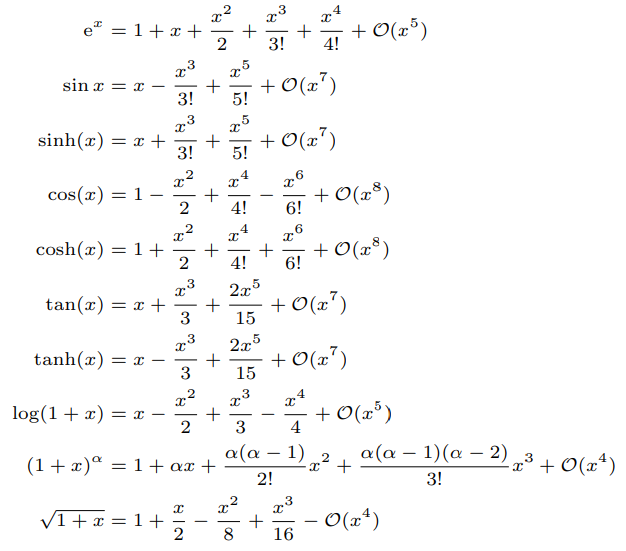
\includegraphics[scale=0.5]{bekannte_taylorreihen.png}
\end{corollary}

\subsubsection{Konvergenz mit Taylorreihen}

\begin{center}
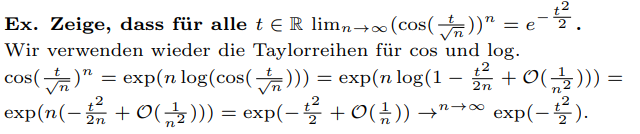
\includegraphics[scale=0.5]{5.png}
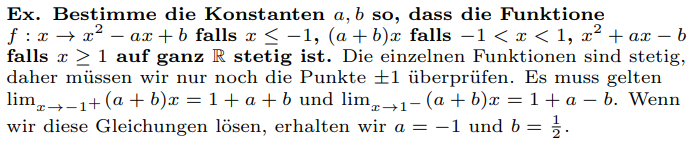
\includegraphics[scale=0.5]{4.png}
\end{center}

	\raggedcolumns
	\pagebreak
	%\section{Integralrechnung}

\subsection{Fundamentalsatz und Stammfunktionen}

\begin{theorem}{Fundamentalsatz der Differential- und Integralrechnung}
    Seien $a<b$ und $f:[a,b] \to \R$ stetig.
    Die Funktion $F(x) = \int_{a}^{x} f(t) \dif t \quad a \leq x \leq b$ ist in $[a,b]$ stetig differenzierbar und $F'(x) = f(x) \quad \forall x \in [a,b]$.
\end{theorem}

\begin{definition}{Stammfunktion}
    Seien $a<b$ und $f:[a,b] \to \R$ stetig.
    Eine Funktion $F: [a,b] \to \R$ heisst \emph{Stammfunktion} von $f$, falls $F$ (stetig) differenzierbar in $[a,b]$ ist und $F' = f$ in $[a,b]$ gilt.

    Die Stammfunktion $F$ von $f$ ist bis auf eine additive Konstante eindeutig bestimmt und es gilt:
    \begin{equation}
        \int_{a}^{b} f(x) \dif x = F(b) - F(a)
    \end{equation}
\end{definition}

\begin{theorem}{Eigenschaften Integrierbarkeit}
    \begin{itemize}
        \item Sei $f : [a,b] \to \R$ \textit{stetig}. Dann ist $f$ integrierbar.
        \item Sei $f: [a,b] \to \R$ \textit{monoton}. Dann ist $f$ integrierbar.
        \item Seien $f,g : [a,b] \to \R$ beschränkt, integrierbar und $\lambda \in \R$.
                Dann sind $f+g$, $\lambda \cdot f$, $f \cdot g$, $|f|$, $\max(f,g)$ und $\frac{f}{g}$
                (falls $|g(x)| \geq \beta > 0 \quad \forall x \in [a,b]$) integrierbar.
        \item Seien $P,Q$ Polynome und $[a,b]$ ein Intervall, in dem $Q$ keine Nullstelle besitzt. Dann ist $[a,b] \to \R$, $x \mapsto \frac{P(x)}{Q(x)}$ integrierbar.
        \item Sind $f, g$ in einer endlichen Menge an Punkten verschieden, sind entweder beide oder keine der Beiden integrierbar.
        \item Sei $f: [a,b] \to \R$ stetig in dem kompakten Intervall $[a,b]$. Dann ist $f$ in $[a,b]$ gleichmässig stetig.
    \end{itemize}
\end{theorem}

\subsection{Unbestimmte und Bestimmte Integrale}

\begin{definition}{Unbestimmtes Integral}
    Sei $f: I \to \R$ auf einem Intervall $I \subseteq \R$ definiert.
    Falls $f$ stetig ist, gibt es eine Stammfunktion $F$ für $f$.
    \begin{equation}
        \int f(x) \dif x = F(x) + C
    \end{equation}
    Das unbestimmte Integral ist die Umkehroperation zur Ableitung.
\end{definition}

\begin{concept}{Integralregeln}
    \begin{itemize}
      \item Addition/Subtraktion:
      $$\int f(x-k) \dif x=F(x-k)+C$$
      \item Multiplikation:
      $$\int f(x \cdot k) \dif x=\frac{1}{k} F(x \cdot k)+C$$
      \item Skalarmultiplikation:
      $$\int \lambda_{1} f(x)+\lambda_{2} g(x) \dif x=\lambda_{1} F(x)+\lambda_{2} G(x)+C$$
    \end{itemize}
\end{concept}

\begin{definition}{Bestimmtes Integral}
    Für ein bestimmtes Integral von $f$ über $[a, b]$ schreibt man:
    \begin{equation}
        \int_{a}^{b} f(x) \dif x
    \end{equation}

    Sei $f(x)$ eine im Intervall $[a, b]$ stetige Funktion:
    \begin{equation}
        F'_{a}(x)=\frac{d}{dx}\left(\int_{a}^{x} f(t) \dif t\right)=f(x)
    \end{equation}

    Sei $f(x)$ eine im Intervall $[a, b]$ stetige Funktion, und sei $F(x)$ eine beliebige Stammfunktion von $f(x)$:
    \begin{equation}
        \int_{a}^{b} f(t) \dif t=F(b)-F(a)
    \end{equation}
\end{definition}

\begin{concept}{Rechnen mit bestimmten Integralen}
    Seien $a < b < c$ und $f: [a,b] \to \R$ beschränkt mit $f|_{[a,b]}$ und $f|_{[b,c]}$ integrierbar, sowie $\lambda_1, \lambda_2 \in \R$. Dann gilt:
    \begin{equation}
        \int_a^c f(x) \dif x = \int_a^b f(x) \dif x + \int_b^c f(x) \dif x
    \end{equation}
    und erweitert (mit Skalaren):
    \begin{equation}
        \int_a^b \left( \lambda_1 f_1 (x) + \lambda_2 f_2 (x) \right) \dif x = \lambda_1 \int_a^b f_1(x) \dif x + \lambda_2 \int_a^b f_2(x) \dif x
    \end{equation}
\end{concept}

\begin{definition}{Riemann-Integrale und Partitionen}
    Eine Partition von $[a,b]$ ist eine endliche Teilmenge $P \subseteq [a,b]$ wobei $\{a,b\} \subseteq P$.

    \textbf{Untersumme}: $s(f,P) \coloneqq \sum_{i=1}^n f_i \delta_i \qquad f_i = \inf\limits_{x_{i-1} \leq x \leq x_i} f(x)$

    \textbf{Obersumme}: $S(f,P) \coloneqq \sum_{i=1}^n F_i \delta_i \qquad F_i = \sup\limits_{x_{i-1} \leq x \leq x_i} f(x)$

    $\delta_i$ bezeichnet die Länge des Teilintervalls.
\end{definition}

\begin{lemma}{Verfeinerung und Menge P}
    \begin{enumerate}
        \item Sei $P'$ eine Verfeinerung von $P$, dann gilt:
            $s(f,P) \leq s (f,P') \leq S(f,P') \leq S(f, P)$
        \item Für beliebige Partitionen $P_1, P_2$ gilt: $s(f,P_1) \leq S(f,P_2)$.
    \end{enumerate}
\end{lemma}

\begin{definition}{Riemann Integrierbar}
    Eine beschränkte Funktion $f : [a,b] \to \R$ ist Riemann integrierbar, falls $s(f) = S(f)$. In diesem Fall bezeichnen wir den gemeinsamen Wert von $s(f)$ und $S(f)$ mit
    $\int_{a}^{b} f(x) \dif x$

    Sei $\mathcal{P}(I)$ die Menge der Partitionen von $I$:
    \begin{equation}
        s(f) = \sup_{P \in \mathcal{P}(I)} s(f,P) \qquad S(f) = \inf_{P \in \mathcal{P}(I)} S(f,P)
    \end{equation}
\end{definition}

\begin{theorem}{Alternative Kriterien}
    Eine beliebige beschränkte Funktion $f$ ist genau dann integrierbar, falls:
    \begin{itemize}
         \item $\forall \varepsilon > 0 ~ \exists P \in \mathcal{P}(I) \quad \text{mit} \quad S(f,P) - s(f,P) < \varepsilon$
    \end{itemize}

    Für $f : [a,b] \to \R$:
    \begin{itemize}
         \item $\forall \varepsilon > 0 ~\exists \delta > 0$ sodass
    $\forall P \in \mathcal{P}_\delta (I), S(f,P) - s(f,P) < \varepsilon$
     \end{itemize}

    Mit $A \coloneqq \int_a^b f(x) \dif x$:
    \begin{itemize}
        \item $\forall \varepsilon > 0 ~ \exists \delta > 0$ sodass $\forall P \in \mathcal{P} (I)$ Partition mit $\delta(P) < \delta$ und $\xi_1 , \ldots , \xi_n$ mit $\xi_i \in [x_{i-1},x_i]$, $P = \{x_0 , \ldots , x_n\}$ gilt:
        $$\left| A - \sum_{i=1}^n f(\xi_i) (x_i - x_{i-1})\right| < \varepsilon$$
    \end{itemize}
\end{theorem}

\subsection{Wichtige Stammfunktionen}

\begin{highlight}{Wichtige Stammfunktionen}
    $\int f(x) \dif x \Longrightarrow F(x) + C$
    \begin{center}
        \begin{minipage}{0.45\linewidth}
            \tcbsubtitle{Potenzfunktionen}
            \begin{align*}
                &\int x^n \dif x  &=&  \quad \frac{1}{n+1}x^{n+1} \quad (n \neq -1) \\
                &\int \frac{f'}{f} \dif x  &=&  \quad \ln \left\lvert f \right\rvert  \\
                &\int \frac{1}{x} \dif x  &=& \quad \ln \left\lvert x \right\rvert  \\
                &\int \frac{1}{x+a} \dif x  &=&  \quad \ln \left\lvert x+a \right\rvert \\
                &\int \frac{1}{(x+a)^2} \dif x  &=&  -\frac{1}{x+a}  \\
                &\int \frac{1}{\sqrt{x}}\dif x  &=&  2 \sqrt{x}  \\
            \end{align*}
        \end{minipage}
        \hfill\vline\hfill
        \begin{minipage}{0.45\linewidth}
            \tcbsubtitle{Exponential- und Logarithmusfunktionen}
            \begin{align*}
                &\int e^{x} \dif x  &=& e^{x} \\
                &\int e^{ax} \dif x  &=&  \frac{1}{a} e^{ax}  \\
                &\int a^{x} \dif x \quad  &=& \frac{a^{x}}{\ln (a)} \\
                &\int \ln (x) \dif x  &=& x \cdot \ln (x)-x \\
                &\int \log_{a}(x) \dif x  &=& \frac{x \cdot \ln (x)-x}{\ln (a)} \\
            \end{align*}
        \end{minipage}
    \end{center}

    \tcbsubtitle{Trigonometrische Funktionen}
    \begin{center}
        \begin{minipage}{0.4\linewidth}
            \begin{align*}
                &\int\cos (x) \dif x  &=& \sin (x) \\
                &\int\sin (x) \dif x  &=& -\cos (x) \\
                &\int\tan (x) \dif x  &=& -\ln |\cos (x)| \\
                &\int \sin(ax)\dif x  &=&  - \frac{1}{a} \cos(a x)  \\
                &\int \sin^2(ax)\dif x  &=&  \frac{x}{2} - \frac{1}{4a} \sin(2 a x)  \\
                &\int \cos(ax)\dif x  &=&  \frac{1}{a} \sin(a x)  \\
                &\int \cos^2(ax)\dif x  &=&  \frac{x}{2} + \frac{1}{4a} \sin(2 a x)  \\
            \end{align*}
        \end{minipage}
        \hfill\vline\hfill
        \begin{minipage}{0.45\linewidth}
            \begin{align*}
                &\int\frac{1}{1+x^{2}} \dif x  &=& \arctan (x)\\
                &\int\frac{1}{\sqrt{1-x^{2}}} \dif x  &=& \arcsin (x) \\
                &\int -\frac{1}{\sqrt{1-x^{2}}} \dif x  &=& \arccos (x) \\
            \end{align*}
        \end{minipage}
    \end{center}
\end{highlight}

\subsection{Rechnen mit Integralen}

\begin{corollary}{Nützliche Regeln}
    Sei $I \subseteq \R$ ein Intervall und $f: I \to \R$ stetig.
    \begin{enumerate}
        \item Seien $a,b,c \in \R$, sodass das abgeschlossene Intervall mit den Endpunkten $a+c$, $b+c$ in $I$ enthalten ist.
            Dann gilt
            \begin{equation}
                \int_{a+c}^{b+c} f(x) \dif x = \int_{a}^{b} f(t+c) \dif t
            \end{equation}
        \item Seien $a,b,c \in \R$ mit $c \neq 0$, sodass das abgeschlossene Intervall mit Endpunkten $ac$, $bc$ in $I$ enthalten ist.
            Dann gilt
            \begin{equation}
                \int_{a}^{b} f(ct) \dif t = \frac{1}{c} \int_{ac}^{bc} f(x) \dif x
            \end{equation}
    \end{enumerate}
\end{corollary}

\begin{concept}{Symmetrie ungerader Funktionen}
    Falls eine Funktion ungerade ist und symmetrische Grenzen hat:
    \begin{equation}
        \int_{-a}^{a} f(x) \dif x = 0 \quad \text{für ungerade } f
    \end{equation}

    Beispiel: $\int_{-\frac{\pi}{2}}^{\frac{\pi}{2}} (\sin x)^7 \cos x \dif x = 0$
\end{concept}

\begin{KR}{Flächeninhalt bei wechselndem Vorzeichen von $f(x)$}
    \begin{itemize}
      \item $[a, b]$ = Intervall
      \item $x_{1}, x_{2}, \ldots, x_{n}$ = Nullstellen
    \end{itemize}

    $$\left|\int_{a}^{x_{1}} f(x) \dif x\right|+\left|\int_{x_{1}}^{x_{2}} f(x) \dif x\right|+\cdots+\left|\int_{x_{n}}^{b} f(x) \dif x\right|$$
\end{KR}

\begin{center}
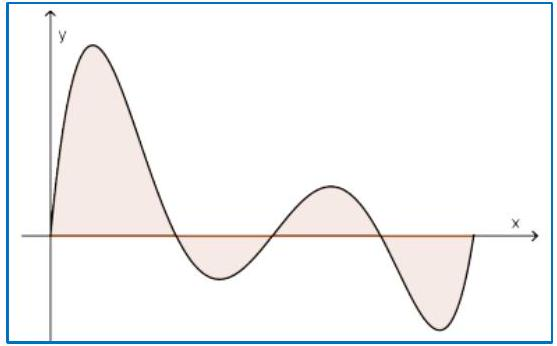
\includegraphics[scale=0.25]{2024_01_20_7bfda6c084929ccc01ffg-06(1).jpg}
\end{center}

\begin{KR}{Flächeninhalt zwischen zwei Kurven $f(x)$ und $g(x)$}
    \begin{itemize}
      \item $[a, b]$ = Intervall
      \item $x_{1}, x_{2}, \ldots, x_{n}$ = Schnittpunkte
    \end{itemize}
    $$\left|\int_{a}^{x_{1}}(f(x)-g(x)) \dif x\right|+\left|\int_{x_{1}}^{x_{2}}(f(x)-g(x)) \dif x\right|+\cdots+\left|\int_{x_{n}}^{b}(f(x)-g(x)) \dif x\right|$$
\end{KR}

\begin{center}
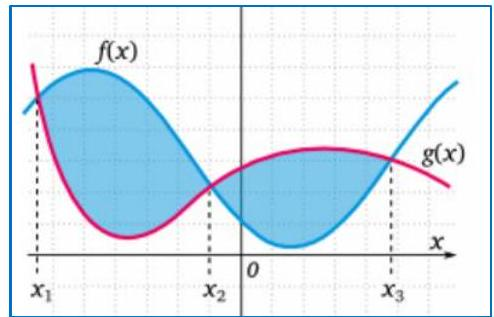
\includegraphics[scale=0.25]{2024_01_20_7bfda6c084929ccc01ffg-06(2).jpg}
\end{center}

\begin{KR}{Strategie zur Berechnung von Integralen}
    \textbf{Bruchform:}
    \begin{enumerate}
        \item Vereinfache, so dass ein einfacher Nenner entsteht
        \item Partialbruchzerlegung
        \item $\frac{u'}{2\sqrt{u}}$ oder $\frac{u'}{u}$ erkennen $\Rightarrow \sqrt{u}$ oder $\ln|u|$
    \end{enumerate}

    \textbf{Produktform:}
    \begin{enumerate}
        \item Partielle Integration anwenden (evtl. mehrmals)
        \item Kettenregel verwenden
    \end{enumerate}

    \textbf{Potenzen:}

    $\int_{a}^{b} f(x)^{c} \dif x$ umformen in $\int_{a}^{b}\left(f(x)^{c} \cdot 1\right) \dif x$ oder $\int_{a}^{b}\left(f(x)^{c-1} \cdot f(x)\right) \dif x$ um dann partielle Integration anzuwenden

    \textbf{Exponentenform:}

    $e / \log$ Trick verwenden, wenn Variable im Exponenten ist.

    \textbf{Produkt mit $e, \sin , \cos$:}

    Mehrmals partielle Integration anwenden, wobei sin, cos immer $g'$ und immer $f$ ist.

    \textbf{Summe im Integral:}

    Summe aus dem Integral herausziehen (dafür muss die Reihe gleichmässig konvergieren)
\end{KR}

\begin{corollary}{Ungleichungen}
    Seien $f,g : [a,b] \to \R$ beschränkt integrierbar:
    \begin{enumerate}
        \item $f(x) \leq g(x) \quad \forall x \in [a,b]$ $\Rightarrow$ $\int_a^b f(x) \dif x \leq \int_a^b g(x) \dif x$
        \item $\left| \int_a^b f(x) \dif x \right| \leq \int_a^b |f(x)| \dif x$
        \item $\left| \int_a^b f(x) g(x) \dif x \right| \leq \sqrt{\int_{a}^{b} f^2(x) \dif x} \sqrt{\int_{a}^{b} g^2(x) \dif x}$
    \end{enumerate}
\end{corollary}

\begin{theorem}[important]{Mittelwertsatz}
    Sei $f:[a,b] \to \R$ stetig.
    Dann gibt es $\xi \in [a,b]$ mit
    \begin{equation}
        \int_{a}^{b} f(x) \dif x = f(\xi)(b-a)
    \end{equation}
\end{theorem}

\begin{theorem}{Folgerung Mittelwertsatz}
    Seien $f,g: [a,b] \to \R$ wobei $f$ stetig, $g$ beschränkt integrierbar mit $g(x) \geq 0~\forall x \in [a,b]$.
    Dann gibt es $\xi \in [a,b]$ mit
    \begin{equation}
        \int_{a}^{b} f(x)g(x) \dif x = f(\xi) \int_{a}^{b} g(x) \dif x
    \end{equation}
\end{theorem}

\subsection{Partielle Integration}

\begin{concept}{Partielle Integration}
    Seien $a < b$ reelle Zahlen und $f,g:[a,b] \to \R$ stetig differenzierbar. Dann gilt
    \begin{equation}
        \int_a^b f(x) g'(x) \dif x = f(b) g(b) - f(a) g(a) - \int_a^b f'(x)g(x) \dif x
    \end{equation}
    bzw. für unbestimmte Integrale
    \begin{equation}
        \int f(x) \cdot g'(x) \dif x = f(x) \cdot g(x) - \int f'(x) \cdot g(x) \dif x
    \end{equation}
\end{concept}

\begin{KR}{Prioritäten für partielle Integration}
    Für die partielle Integration $f(x)$ nach folgender Priorität auswählen:
    \begin{center}
    \begin{tabular}{lll}
        1. $\log_e, \log_a$  &  3. $x^2, 5x^3$ & 5. $e^x, 5a^x$\\
        2. $\arcsin, \arccos$ & 4. $\sin, \cos, \tan$ &
    \end{tabular}
    \end{center}
\end{KR}

\begin{remark}
    $\uparrow$ 1 falls arc- oder log-Funktion vorkommt, $x^{n}, \frac{1}{1-x^{2}}, \frac{1}{1+x^{2}}$

    $\downarrow$ $x^{n}, \arcsin (x), \arccos (x), \arctan (x)$
\end{remark}

\subsection{Substitution}

\begin{concept}{Substitution}
    Die Substitution ist die Umkehrung der Kettenregel. D.h. wir wollen Substitution vorallem verwenden, wenn wir innere Funktionen haben.
    \begin{equation}
        \int_{a}^{b} f(g(t)) g'(t) \dif t = \int_{g(a)}^{g(b)} f(x) \dif x
    \end{equation}
    bzw. für unbestimmte Integrale
    \begin{equation}
        \int f(g(t)) \cdot g'(t) \dif t=\left.\int f(x) \dif x\right|_{x=g(t)}
    \end{equation}
\end{concept}

\begin{formula}{Nützliche Substitutionen}
    \begin{itemize}
        \item $e^{x}, \sinh (x), \cosh (x)$, subst: $t=e^{a x}, \dif x=\frac{\dif t}{a t}$. Dann $\sinh = \cosh = \frac{t^{2}-1}{2 t}$
        \item $\log (x)$ subst: $t=\log (x), x=e^{t}, \dif x=e^{t} \dif t$
        \item für gerade $n: \cos^{n}(x), \sin^{n}(x), \tan (x)$ Sub: $t=\tan (x)$, $\dif x=\frac{1}{1+t^{2}} \dif t, \sin^{2}(x)=\frac{t^{2}}{1+t^{2}}, \cos^{2}(x)=\frac{1}{1+t^{2}}$
        \item für ungerade $n: \cos^{n}(x), \sin^{n}(x)$, Sub: $t=\tan (x / 2)$, $\dif x=\frac{2}{1+t^{2}} \dif t, \sin (x)=\frac{2 t}{1+t^{2}}, \cos (x)=\frac{1-t^{2}}{1+t^{2}}$
        \item $\int \sqrt{1-x^{2}} \dif x$ sub: $x=\sin (x)$ oder $\cos (x)$
        \item $\int \sqrt{1+x^{2}} \dif x$ sub: $x=\sinh (x)$
    \end{itemize}
\end{formula}

\begin{example}
    Bsp. $\int \frac{x}{\sqrt{9-x^{2}}} \dif x$ substitution mit $t=\sqrt{9-x^{2}}$.

    $$\Rightarrow x=\sqrt{9-t^{2}} \Rightarrow x'=\frac{-2 t}{2 \sqrt{9-t^{2}}} \Rightarrow \dif x=\frac{-t \cdot \dif t}{\sqrt{9-t^{2}}}$$

    $\int-\dif t=-t$ rücksubstitution $\Rightarrow-\sqrt{9-x^{2}}$
\end{example}

\subsection{Partialbruchzerlegung}

\begin{KR}{Stammfunktionen rationaler Funktionen}
    Die Stammfunktion einer Funktion $R(x)=\frac{P(x)}{Q(x)}$ bestehend aus rationalen Funktionen lässt sich als eine Funktion von Polynomen, rationalen, exponentiellen, logarithmischen, trigonometrischen und inversen trigonometrischen Funktionen darstellen.

    Zuerst wollen wir, dass $\grad(P)<\grad(Q)$ gilt, falls dies nicht der Fall ist, führen wir Polynomdivision aus. Danach bestimmen wir alle reellen und komplexen Nullstellen. Nun gilt:

    $$R(x)=\sum_{k=1}^{N} R_{k}(x)+\sum_{k=1}^{M} Q_{k}(x)$$

    Hier ist $N$ die Anzahl reeller Nullstellen und $M$ die Anzahl der komplexen Nullstellen. Es gilt:

    $$\begin{gathered}
    R_{k}(x)=\frac{a_{k_{1}}}{(x-x_{k})}+\frac{a_{k_{2}}}{(x-x_{k})^{2}}+\ldots+\frac{a_{k_{n_{k}}}}{(x-x_{k})^{n_{k}}} \\
    Q_{k}(x)=\frac{a_{k_{1}}+b_{k_{1}} x}{((x-\alpha_{k})^{2}+\beta_{k}^{2})}+\ldots+\frac{a_{k_{m_{k}}}+b_{k_{m_{k}}} x}{((x-\alpha_{k})^{2}+\beta_{k}^{2})^{m_{k}}}
    \end{gathered}$$

    Somit können wir die Funktion mit Partialbruchzerlegung in einzelne Brüche darstellen, welche dann leichter zu integrieren sind. Wenn wir eine reelle Nullstelle haben, so gilt:

    $$\int \frac{1}{(x-\gamma_{i})^{n}} \dif x =\begin{cases}
    \ln (x-\gamma_{i}) & \text{für } n=1 \\
    \frac{-1}{(n-1)(x-\gamma_{i})^{n-1}} & \text{für } n > 1
    \end{cases}$$

    Für komplexe Nullstellen gilt:

    $$\begin{gathered}
    \frac{A+B x}{((x-\alpha)^{2}+\beta^{2})^{j}}=\frac{B(x-\alpha)}{((x-\alpha)^{2}+\beta^{2})^{j}}+\frac{A+B \alpha}{((x-\alpha)^{2}+\beta^{2})^{j}} \\
    \int \frac{B(x-\alpha)}{((x-\alpha)^{2}+\beta^{2})^{j}} \dif x =\begin{cases}
    \frac{B}{2} \ln ((x-\alpha)^{2}+\beta^{2}) & \text{für } j=1 \\
    \frac{B}{(2(1-j))((x-\alpha)^{2}+\beta^{2})^{j-1}} & \text{für } j > 1
    \end{cases}
    \end{gathered}$$

    Für den letzten Term brauchen wir die Substitution $(x-\alpha)=\beta t$:

    $$\int \frac{A+B \alpha}{((x-\alpha)^{2}+\beta^{2})^{j}} \dif x=\frac{A+B \alpha}{\beta^{2 j-1}} \cdot \int \frac{1}{(t^{2}+1)^{j}} \dif t$$
\end{KR}

\begin{example}
    Bsp.
    $$\int \frac{x^{2}-x+2}{x^{3}-x^{2}+x-1} \dif x$$

    Wir finden die erste Nullstelle $(x-1)$ durch Ausprobieren. Danach führen wir Polynomdivision (durch $x-1$) aus und erhalten damit die weitere Nullstelle $(x^{2}+1)$. Da $x^{2}+1$ eine komplexe Nullstelle ist, nehmen wir dafür $A+B x$:

    $$\frac{A+B x}{x^{2}+1}+\frac{C}{x-1}=\frac{x^{2}-x+2}{(x^{2}+1)(x-1)}$$

    $\Longrightarrow x^{2}-x+2=(A+C) \cdot x^{2}+(B-A) x+(C-B) \cdot 1$

    $\Longrightarrow B=0, A=-1, C=1$

    $\Longrightarrow \int \frac{1}{x-1}+\frac{-1}{x^{2}+1} \dif x=\ln (x-1)-\arctan (x)+C$
\end{example}

\begin{corollary}{Reduktionsformel}
    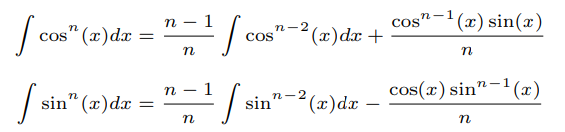
\includegraphics[scale=0.5]{reduktionsformel.png}
\end{corollary}

\subsection{Uneigentliche Integrale und weitere Themen}

\begin{theorem}[important]{Euler-McLaurin Summenformel}
    Wird verwendet, um Summen (wie $\sum_{i=1}^n \frac{1}{i}$, $\sum_{i=1}^n \ln{i}$ oder $\sum_{i=1}^n i^\ell$) abzuschätzen.

    Sei $f : [0,n] \to \R$ $k$-mal stetig differenzierbar, $k \geq 1$.
    Dann gilt:
    \begin{enumerate}
        \item Für $k=1$:
        \begin{equation}
            \sum^{n}_{i=1} f(i) = \int_{0}^{n} f(x) \dif x + \frac{1}{2} ( f(n) - f(0) ) + \int_{0}^{n} \tilde{B}_1 (x) f'(x) \dif x
        \end{equation}
        \item Für $k \geq 2$:
        \begin{align}
            \sum^{n}_{i=1} f(i) &= \int_{0}^{n} f(x) \dif x + \frac{1}{2} ( f(n) - f(0) )\\
            &+ \sum^{k}_{j=2} \frac{(-1)^j B_j}{j!} ( f^{(j-1)} (n) - f^{(j-1)} (0) ) + \tilde{R}_k
        \end{align}
        wobei $\tilde{R}_k = \frac{(-1)^{k-1}}{k!} \int_{0}^{n} \tilde{B}_k (x) f^{(k)} (x) \dif x$
    \end{enumerate}
\end{theorem}

\begin{highlight}{Potenzsummen}
    Für Potenzsummen der Form $1^l + 2^l + \ldots + n^l$ wobei $l \geq 1, l \in \N$ kann die Summenformel mit $f(x) = x^l$ und $k=l+1$ angewendet werden.
    Daraus folgt für alle $l \geq 1$:
    \begin{equation}
        1^l + 2^l + \ldots + n^l = \frac{1}{l+1} \sum^{l}_{j=0} (-1)^j \begin{pmatrix}l+1\\j\end{pmatrix} B_j n^{l+1-j}
    \end{equation}
\end{highlight}

\begin{concept}{Integration konvergenter Reihen}
    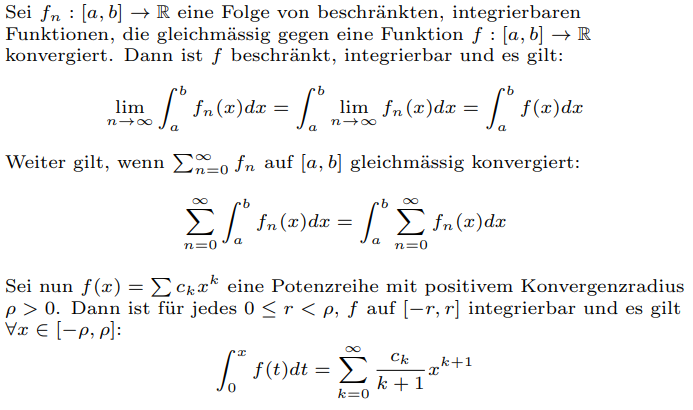
\includegraphics[scale=0.5]{integration_konvergenter_reihen.png}
\end{concept}

\begin{lemma}{Holder'sche Ungleichung}
    Sei $p > 1$ und $q > 1$ mit $\frac{1}{p} + \frac{1}{q} =1$.
    Dann gilt $\forall a,b \geq 0$:
    \begin{equation}
        a \cdot b \leq \frac{a^p}{p} + \frac{b^q}{q}
    \end{equation}
\end{lemma}

\begin{theorem}{Verallgemeinerung Holder'sche Ungleichung}
    Seien $p > 1$ und $q> 1$ mit $\frac{1}{p} + \frac{1}{q} = 1$.
    Für alle $f,g : [a,b] \to \R$ stetig gilt:
    \begin{equation}
        \int_{a}^{b} |f(x) g(x)| \dif x \leq ||f||_p ||g||_q
    \end{equation}
    wobei $||f||_p \coloneqq \left( \int_{a}^{b} |f(x)|^p \dif x \right)^{\frac{1}{p}}$
\end{theorem}

	\raggedcolumns
\end{multicols}
\end{document}